\documentclass[a4paper,12pt]{article}

\usepackage[table,xcdraw]{xcolor}
\usepackage{graphicx}
\usepackage{microtype}
\usepackage{vhistory}
\usepackage{subfig}
\usepackage[T1]{fontenc}
\usepackage{lmodern}
\usepackage[nolist,nohyperlinks]{acronym}
\usepackage{hyperref}
\usepackage[absolute,overlay]{textpos}
\usepackage[edges]{forest}
\usepackage{tikz}
\usepackage{flexisym}
\usepackage[outputdir=build]{minted}
\usepackage{longtable}
\usepackage{booktabs}


\usepackage{array}
\newcolumntype{M}[1]{>{\centering\arraybackslash}m{#1}}

\usepackage{makecell}
\renewcommand{\cellalign}{l}

\graphicspath{ {resources/} }

\hypersetup{
    colorlinks,
    linkcolor={black},
    citecolor={black},
    urlcolor={blue!80!black}
}

\definecolor{eclipseStrings}{RGB}{42,0.0,255}
\definecolor{eclipseKeywords}{RGB}{127,0,85}
\colorlet{numb}{magenta!60!black}


\definecolor{leaf_green}{RGB}{182,215,168}
\definecolor{composite_yellow}{RGB}{255,229,154}
\definecolor{decorator_purple}{RGB}{179,168,210}
\definecolor{decision_red}{RGB}{221,124,110}

\usepackage[margin=1in]{geometry}

\forestset{
composite/.style={rectangle,fill=composite_yellow,draw,rounded corners,thick},
leaf/.style={rectangle,fill=leaf_green,draw,rounded corners,thick},
decorator/.style={rectangle,fill=decorator_purple,draw,rounded corners,thick},
decision/.style={rectangle,fill=decision_red,draw,rounded corners,thick}
}

\usepackage{listings}
\usepackage{courier}
\lstset{
    basicstyle=\footnotesize\ttfamily, % Default font
    numbers=left,              % Location of line numbers
    numberstyle=\tiny,          % Style of line numbers
    % stepnumber=2,              % Margin between line numbers
    numbersep=5pt,              % Margin between line numbers and text
    tabsize=2,                  % Size of tabs
    extendedchars=true,
    breaklines=true,            % Lines will be wrapped
    %keywordstyle=\color{red},
    frame=b,
    %keywordstyle=\color{blue},
    %stringstyle=\color{red},
    %commentstyle=\color{green},
    %morecomment=[l][\color{magenta}]{\#},
    %stringstyle=\color{white}\ttfamily, % Color of strings
    showspaces=false,
    showtabs=false,
    xleftmargin=17pt,
    framexleftmargin=17pt,
    framexrightmargin=5pt,
    framexbottommargin=4pt,
    % backgroundcolor=\color{lightgray},
    showstringspaces=false
}
\lstloadlanguages{ % Check documentation for further languages ...
      C++,
      bash,
      XML
}

% \DeclareCaptionFont{blue}{\color{blue}} 

% \captionsetup[lstlisting]{singlelinecheck=false, labelfont={blue}, textfont={blue}}
\usepackage{caption}
\DeclareCaptionFont{white}{\color{white}}
\DeclareCaptionFormat{listing}{\colorbox[cmyk]{0.43, 0.35, 0.35,0.01}{\parbox{\textwidth}{\hspace{15pt}#1#2#3}}}
\captionsetup[lstlisting]{format=listing,labelfont=white,textfont=white, singlelinecheck=false, margin=0pt, font={bf,footnotesize}}

\lstdefinelanguage{json}{
    basicstyle=\normalfont\ttfamily,
    commentstyle=\color{eclipseStrings}, % style of comment
    stringstyle=\color{eclipseKeywords}, % style of strings
	numbers=none,
	frame=none,
    stepnumber=1,
    numbersep=8pt,
    showstringspaces=false,
    breaklines=true,
    %backgroundcolor=\color{gray}, %only if you like
    string=[s]{"}{"},
    comment=[l]{:\ "},
    morecomment=[l]{:"},
    literate=
        *{0}{{{\color{numb}0}}}{1}
         {1}{{{\color{numb}1}}}{1}
         {2}{{{\color{numb}2}}}{1}
         {3}{{{\color{numb}3}}}{1}
         {4}{{{\color{numb}4}}}{1}
         {5}{{{\color{numb}5}}}{1}
         {6}{{{\color{numb}6}}}{1}
         {7}{{{\color{numb}7}}}{1}
         {8}{{{\color{numb}8}}}{1}
         {9}{{{\color{numb}9}}}{1}
}


\begin{acronym}
\acro{BT}{Behavior Trees}
\acro{FSM}{Finite State Machines}
\acro{SRL}{Service Robotics Lab}
\end{acronym}

\begin{document}

\date {}
\author{}
\title{Behavior Trees Framework for ROS}

\begin{figure}[ht!]

\includegraphics[width=.3\textwidth]{upo_logo.png}\hfill

\includegraphics[width=.3\textwidth]{tri_logo.png}\hfill

\includegraphics[width=.2\textwidth]{srl_logo.png}
\end{figure}

\begin{textblock*}{10cm}(5.5cm,11cm)
CONFIDENTIAL: FOR INTERNAL USE ONLY
\end{textblock*}

\maketitle

\clearpage
\begin{versionhistory}
\vhEntry{0.1}{22.01.19}{\'{A}lvaro P\'{a}ez}{created}
\end{versionhistory}

\clearpage
\listoffigures

\clearpage
\listoftables

\clearpage
\renewcommand{\lstlistingname}{Code Snippet}
\renewcommand\listoflistingscaption{List of \lstlistingname s}
\listoflistings

\clearpage
\tableofcontents

\clearpage
\section{Overview}
\label{sec:overview}

\ac{BT} are a way to structure the flow and control of multiple tasks in the context of decision-making applications. They are usually presented as an alternative to \ac{FSM}. First originated as a tool for NPC AI development in the video game industry, \ac{BT} have become widespread in robotics, mainly due to its modularity and simplicity \cite{TRO17Colledanchise}.

This document aims to serve both as a technical description and as user documentation on how to make use of behavior trees in a ROS environment. First, a basic introduction to \ac{BT} is presented, mainly to establish terms and conventions that will be used throughout the document. After that, the general structure and the envisioned work-flow is described. Users looking for a quick reference may focus on the following sections, where a descriptive list of all the ready-to-use nodes is presented. A cookbook is also included, with several how-to's and pitfalls behavior designers may encounter. Finally, annexes include more in-depth descriptions on how stuff work under the hood, and rationale behind some decisions taken during development.

\clearpage
\section{Introduction to Behavior Trees}
\label{sec:behavior-trees-introduction}

\ac{BT} model behaviors as hierarchical trees made up of nodes. Trees are traversed from top to bottom at a given rate following a set of well-defined rules and executing the tasks/commands that are encountered while doing so.

Tasks and commands statuses are reported back up in the chain and the flow changes accordingly. A status can be either success, failure or running. It's important to note that these statuses are not associated to a single node, but rather to a parent-child link. This means that parents always get a status coming up through their links, whether what's at the other side it's a single node or a sub-tree. 

According to their functionality, nodes can be classified as:

\begin{itemize}
\item \textbf{Composite}: control the flow through the tree itself and are similar to control structures such as if, while or for loops in traditional programming languages  The most common are:
\begin{itemize}
\item Sequence: loops through its children nodes sequentially. It returns success only if all its children return it as well, otherwise returns fail or running. Similar to an AND gate.
\item Selector: sequence's counterpart. It checks each child node in order until one returns success and halts its processing. It can be thought as an OR gate.
\end{itemize}
\item \textbf{Decorator}: process or modify the status it receives from its child (it can only have one). An example of this would be the Inverter, that returns the opposite status it receives (e.g. fail in case of success and vice versa).
\item \textbf{Leaf}: this is where the actual task is performed and commands defined by the user are executed. As such, these nodes cannot have any children.
\end{itemize}

As it can be seen from the classification above, \ac{BT} decouple logic from actual tasks in a natural way. When developing a tree one only should care about the leaf nodes. The flow can later be defined and re-arranged constantly, creating new behaviors and expanding on what's already done.

\begin{figure}[ht!]
\centering
\begin{forest}
  forked edges,
  [Sequence,composite,calign=child,calign primary child=2
    [Walk to Door,leaf]
    [Selector,composite,calign=child,calign primary child=2
      [Open Door,leaf]
      [Sequence,composite
      	[Unlock Door,leaf]
      	[Open Door,leaf]
      ]
      [Smash Door,leaf]
    ]
    [Walk through Door,leaf]
  ]
\end{forest}
\caption{Example of a simple Behavior Tree representing the sequences of actions to open a door.}
\label{figure:behavior-tree-open-door}
\end{figure}

A simple \ac{BT} listing the sequence of tasks for a given AI to open a door is depicted in figure \ref{figure:behavior-tree-open-door}. Composites are represented as yellow nodes and leaves as green nodes. The well-defined behavior of composites makes it fairly easy to understand how and in what order the different tasks are performed. The root sequence composite ensures, for example, that the "open door" task will not be started until the "walk to door" task is finished with a success status. On the other hand, selector composites can be seen as a mechanism to list optional ways to undergo a task, going from the most to the least favorable. For example, if it is possible to open the door normally, the first child node will return true and the selector processing will come to halt, returning true to its parent and thus resuming the top sequence (it will not try to smash it).

\clearpage
\section{Behavior Trees in ROS}
\label{sec:behavior-trees-ros}

This section shows how to set things up to get trees up and running in your ROS environment. This includes all external dependencies, packages and tools needed to effectively work with them. Several tutorials and examples are included as well. At the end of this section you should be able to create, modify and monitor them at ease.

Trees examples in the following subsections come with default values for topics and other variables. This tutorial assumes you are using the exact same tree with the same values.

\subsection{Setting Things Up}
\label{subsec:setting-up}
There are several libraries and tools that need to be present in the system before you can start working with trees:

\begin{itemize}
\item \textbf{BehaviorTree.CPP}: core library containing the basic functionality. It manages tree navigation and offers some basic default blocks as well as a plugin system.
\item \textbf{Groot}: \textit{BehaviorTree.CPP}-compliant graphical editor. It's possible to create, modify and monitor in real time trees made using the above-mentioned library.
\item \textbf{ZeroMQ}:  high-performance asynchronous messaging library. Not mandatory per se, but \textit{Groot}'s real time monitoring relies on this.
\item \textbf{behavior_tree_ros}: interface package between ROS and \textit{BehaviorTree.CPP}. It offers seamless publication and subscription, a plugin containing some general nodes to manipulate messages and a general node to run trees.
\item \textbf{Other plugins}: external plugins may offer new functionalities or they could serve as an interface for a given system. For example, a plugin for a particular robot could export publishers and subscribers for its custom messages. These plugins can be compiled and imported in \textit{Groot}, thus allowing for an easy adoption. There is currently a repository in the group called \textbf{behavior_tree_plugins} where some plugins are already shipped.
\end{itemize}

Please note that, while \textit{BehaviorTree.CPP} and \textit{Groot} are external dependencies and have a public github repository maintained by the original author, \ac{SRL} has their own fork. Several new features still not implemented upstream have been added, and some upstream changes may not be completely supported yet by the rest of ROS-related packages. As such, the remaining of this document assumes the fork\footnote{\ac{SRL} work is always added on the \textit{upo} branch. \textit{master} and \textit{develop} branches are copies of their upstream counterparts and thus should be avoided.} is being used, and no distinction between custom features and those supported on the original repository is made.

\noindent Before going any further, install \textit{ZeroMQ} using the following command:

\lstinputlisting[label={listing:zmq-install},caption=Installing dependencies,numbers=none]{snippets/install_zmq.bash}

\textit{BehaviorTree.CPP} and \textit{Groot} forks can be found in the group's repository under the same names. They are compiled as any other CMake project\footnote{Keep in mind that, while compilation using catkin is supported, its use is discouraged, due to some changes in the fork}:

\lstinputlisting[label={listing:compile-dependencies}, caption=Compiling packages,numbers=none]{snippets/compile.bash}

\textit{BehaviorTree.CPP} should be installed at the system level rather than just compiled. Consider installing using \textit{sudo make install}. Finally, \textit{behavior_tree_ros} and plugins in \textit{behavior_tree_plugins} repos are normal ROS packages and follow the usual compilation procedure, but they depend on a few packages. Install them before trying to compile:

\lstinputlisting[label={listing:install-dependencies}, caption=Installing \textit{behavior_tree_ros} dependencies,numbers=none]{snippets/install_package_dependencies.bash}

\clearpage
\subsection{Hello World!}
\label{subsec:hello-world}

Let's create our very own first tree. Programming tutorials usually starts off with a \textit{Hello World!} example, and this document is no exception.

Start by creating a new catkin package. Your \textit{CMakeLists.txt} should look like snippet \ref{listing:basic-cmake}.

\lstinputlisting[label={listing:basic-cmake}, caption=Importing \textit{behavior_tree_ros} in cmake,language=XML]{snippets/hello_world_cmake.txt}

Fancy cmake details aside, the only thing that has to be done to use trees in ROS is to include the \textit{behavior_tree_ros} package (see line 19).
Now we have to include some code. While pretty much all the heavy lifting to publish, receive and (de)serialize messages is done \textit{automagically} for you, the package needs to know at compile time what messages you intend to use. Line 25 compiles a library whose only source file is called \textit{plugin.cpp}. Snippet \ref{listing:hello-world-plugin} shows the contents of this file.

\lstinputlisting[label={listing:hello-world-plugin}, caption=Declaring a publisher in a plugin]{snippets/hello_world_plugin.cpp}

A standard string message publisher is instantiated in line 10. By using the templates exposed in the package \textit{behavior_tree_ros} one can easily define a leaf node that will publish a given message every time is executed.

The code has to be compiled as a \textit{BehaviorTree.CPP}-compliant plugin. A full explanation on how the plugin system works is out of the scope of this document (refer to the official online documentation instead \cite{faconti_2019}). Nevertheless, plugins always have this same exact boilerplate code, so the snippet can be used as a template.


We now have one of the building blocks of our behavior tree containing the functionality (in this case, a single \textit{String} publisher). The next step is to define what blocks are interconnected and how should the tree be traversed. For this we are going to use \textit{Groot}.

Launch it and select \textit{Editor} in the splash screen (see Figure \ref{subfig:groot-splash-screen}). You should be presented with an empty workspace. On the left you can see the list of available blocks you may use to build your tree by dragging and dropping them into said workspace.

You can also define manually custom nodes by pressing the first button on top of the node list. A pop-up window should appear, where you can input the name, type and ports of the new node. This method is, however, tedious and error-prone, as the block definition you enter manually has to match those defined in the code of the block itself.

\begin{figure}[ht!]
\centering
\subfloat[Splash screen.]{\label{subfig:groot-splash-screen}
\includegraphics[width=0.41\textwidth]{groot-splash-screen.png}}
\qquad
\subfloat[Empty workspace.]{\label{subfig:groot-empty-workspace}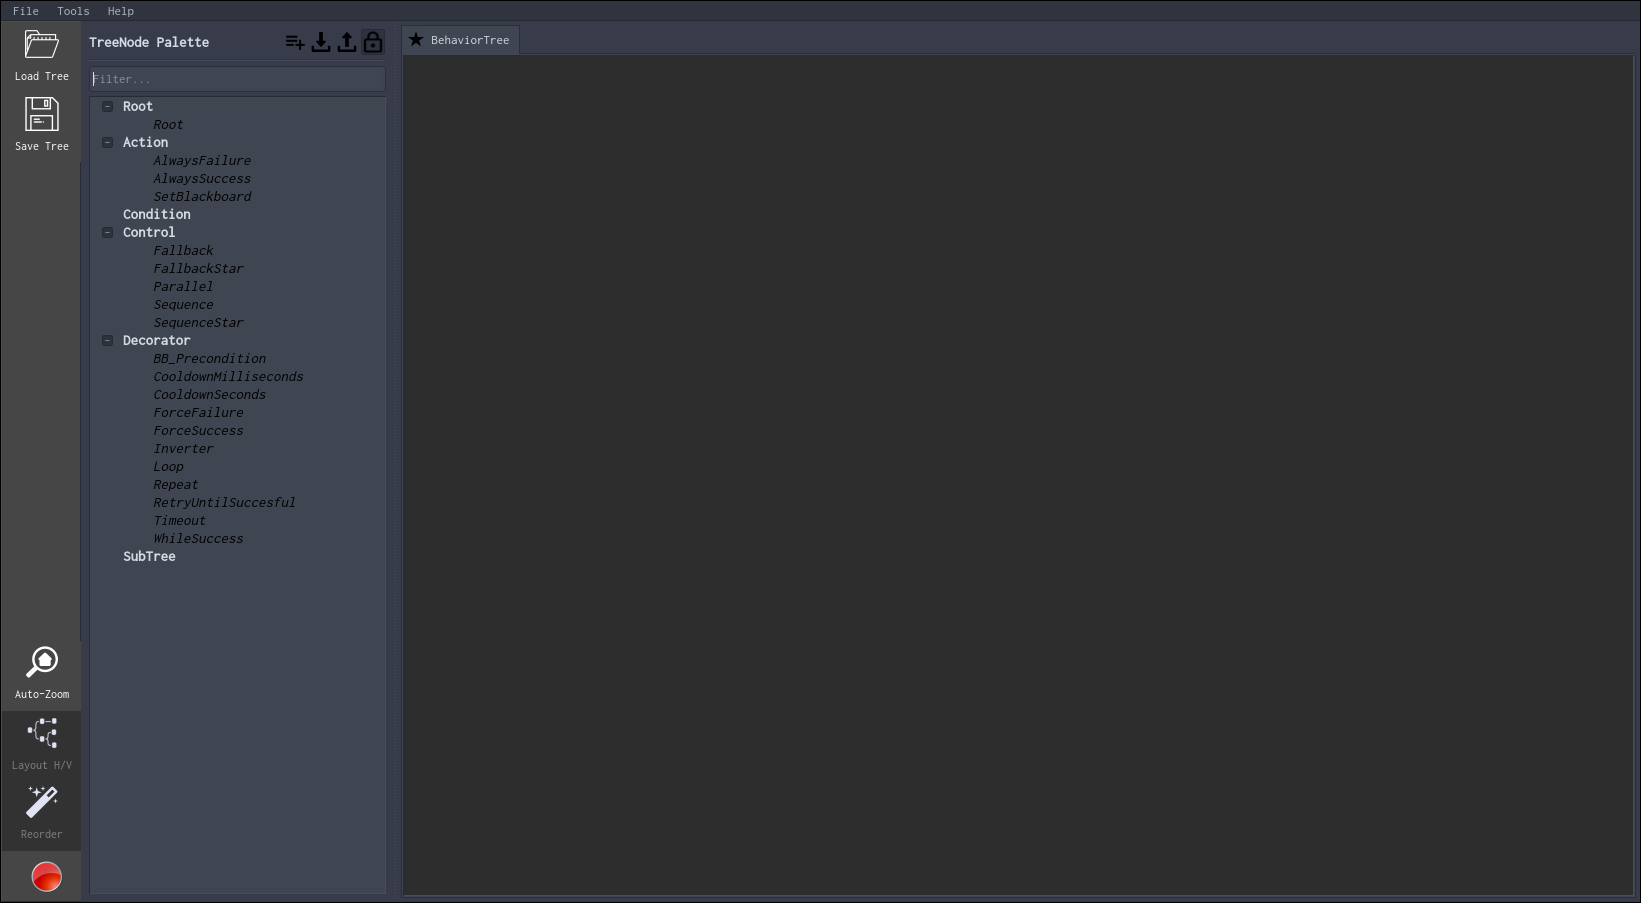
\includegraphics[width=0.49\textwidth]{groot-empty-editor.png}}
\caption{Groot splash screen and empty workspace}
\label{figure:groot-start-screens}
\end{figure}

Rather than doing that, we are going to import the plugin you just compiled. This plugin not only contains the actual execution code, but also nodes' definition and all the info \textit{Groot} needs. Click on the \textit{Load Tree} button in the upper-left. From this menu you can import either behavior tree files in XML format (more on this later) or you can change the type in the bottom dropdown to plugins with a .so extension. The plugin should be in /path/to/workspace/devel/lib/.

After importing the plugin, the string publisher should have appeared in the list under the sames name used in the code (refer back to the snippet \ref{listing:hello-world-plugin}). The resulting tree is shown in Figure \ref{figure:hello-world-tree}. You can find all the blocks you need in the list on the left, or you can type their names in the search bar on top of it.

\begin{figure}[ht!]
\centering
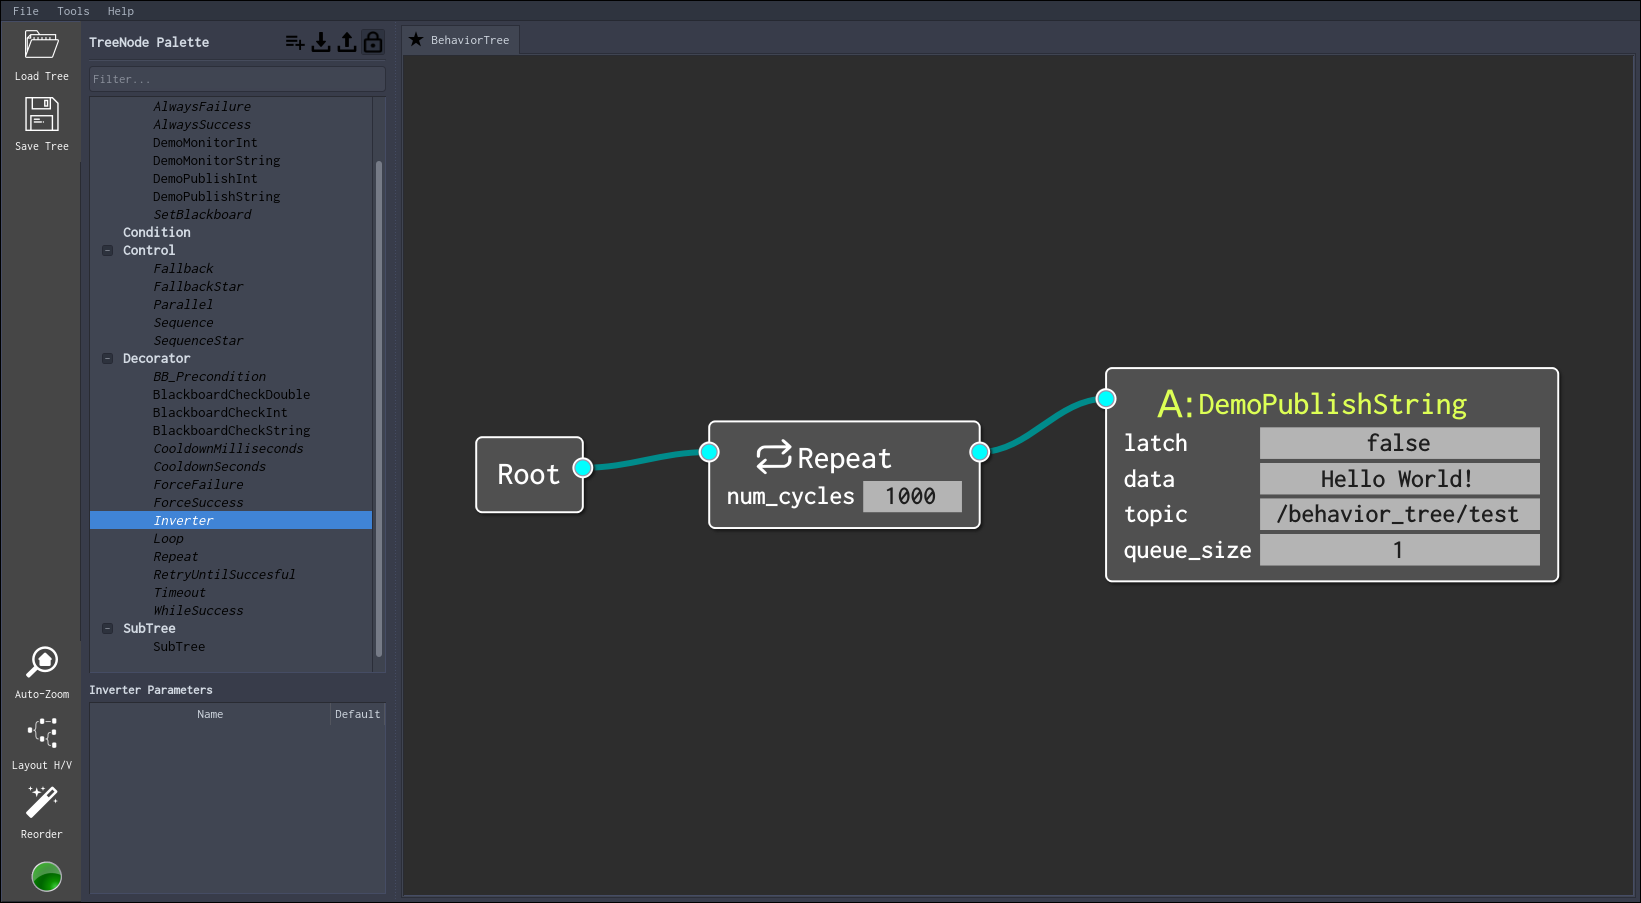
\includegraphics[width=\textwidth]{hello_world.png}
\caption{\textit{Hello World!} tree}
\label{figure:hello-world-tree}
\end{figure}

Let's take a closer look. The tree starts with a \textit{root} node. Trees should always have a \textit{root} as their first block. This connects with a \textit{repeat} node, that has an input parameter to change the maximum number of tries. This block will keep ticking\footnote{The term \textit{tick} is used when a parent node calls the code contained in its child block. Internally, each block has a \textit{tick()} function that defines what it actually does.} its child as long as it returns SUCCESS. The \textit{repeat} node itself will return SUCCESS if it has ticked successfully its child \textit{num_cycles} times or FAILURE if not.

Finally, the last leaf node contains the actual user code. It will publish a message to the topic set in its port every time its ticked.

Click the save button on the left, and you will be prompted to save a file with an XML extension. The contents of the exported file should be similar to those of snippet \ref{listing:hello-world-xml}. It's easy to spot the tree structure, defined in the section enclosed by the <BeahviorTree> tags. The <TreeNodesModel> tags declares the interfaces (input and output ports) of the non-default blocks present in \textit{Groot} when the tree was exported, even if they were not actually used in the tree. The full XML schema and some documentation can be found in the official github repository.

\lstinputlisting[label={listing:hello-world-xml}, caption=\textit{Hello World!} tree XML file]{snippets/hello_world.xml}

Now we have the code defining what the nodes actually do (the plugin), and how these nodes are interconnected (the XML file). The next step is to execute it. The package \textit{behavior_tree_ros} also includes a general node capable of executing trees. Before launching it, all the needed plugins should be placed in /path/to/behavior_tree_ros/resources/plugins/. At startup, the node will scan this folder for plugins and include all the nodes defined in them. Trying to run a tree that uses nodes not loaded will result in an error.

Once the plugin is placed in the directory\footnote{You can use symlinks too, so you don't have to copy the plugins over every time you recompile them.}, you can start the node using the following command:

\lstinputlisting[label={listing:launching-ros-tree},caption=Launching \textit{behavior_tree_ros} node,numbers=none]{snippets/launch_tree_node.bash}

You should see a message stating that it managed to load the plugin. Trees can be run by importing the XML file into the node. Launch the tree with the command below:

\lstinputlisting[label={listing:loading-tree},caption=Loading a tree,numbers=none]{snippets/load_tree.bash}

If everything went fine, you should get some output in the terminal, with the current block in the tree being executed and its result. You can check using rostopic that messages containing the string \textit{Hello World!} are being published in the topic you input in the publisher node's port.

While this tree is far from fancy, the example illustrates the basic work-flow and how to proceed when introducing trees in a new ROS system. To sum it up:

\begin{itemize}
\item Define your leaf nodes in a plugin. They may be publishers and subscribers using custom messages or they can perform some other operations/checks.
\item Import all the plugins containing the blocks you need in Groot.
\item Build your tree and export it as an XML file.
\item Put all the used plugins in the default ROS node folder so they are loaded at start up.
\item Load the XML file using the ROS service.
\end{itemize}

And that's all. No matter how big your tree may be, these steps are always the same.

\subsection{Adding Logic to your Trees}
\label{subsec:trees-logic}

Let's spice things up a bit. To build more complex behaviors we need input data. This data usually take the form of ROS messages received from topics we would like to monitor. We also need to make decisions based on this information, usually by checking values and exploring the data inside the message.

One approach to this is to build custom leaf nodes that work on messages of a given message type. This does not escalate so well, as it would mean you would have to write custom nodes every time you want to manipulate some message. To avoid this, \textit{behavior_tree_ros} subscriber leaf nodes can serialize the messages they receive into a more general structure, allowing for more general-purpose smaller blocks capable of inspecting and performing operations on these messages.

Let's put this to test by building a simple tree that, given a custom user message containing two numbers, it tells us which one is bigger. For the sake of the example, we are going to assume that whoever defined the message had a bad day and did it as shown in the snippet \ref{listing=two-numbers-message}. But worry not, for introspection is here to save the day.

\lstinputlisting[label={listing=two-numbers-message},caption=\textit{TwoNumbers} message definition,numbers=none]{snippets/TwoNumbers.msg}

Add the message to your package and cmake file. A new leaf node to subscribe to this new message should be added in the plugin as well. Modify the \textit{plugin.cpp} file as shown in snippet \ref{listing:plugin-subsriber}.

\lstinputlisting[label={listing:plugin-subsriber},caption=Declaring a subscriber in a plugin]{snippets/two_numbers_plugin.cpp}

Recompile it and import it in Groot. The new tree containing the logic to compare the numbers is shown in figure \ref{figure:example-tree-two_numbers}. Things have gotten a bit more complicated now, so let's go step by step. 

\begin{figure}[ht!]
\centering
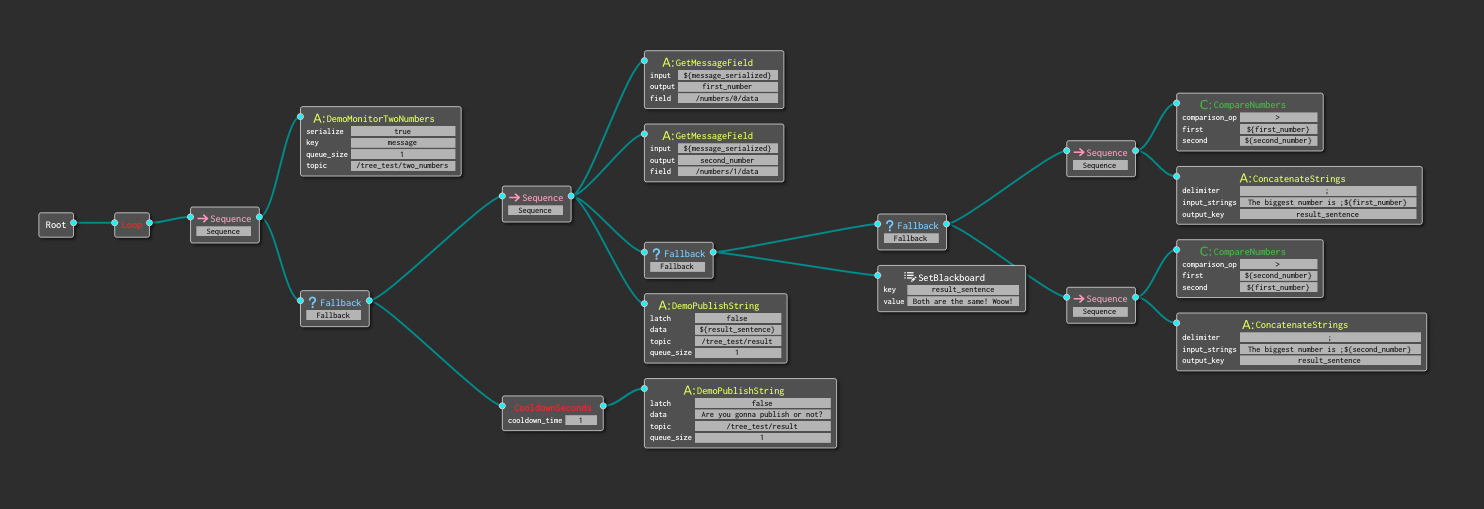
\includegraphics[width=\textwidth]{two_numbers_demo.png}
\caption{Tree comparing two numbers}
\label{figure:example-tree-two_numbers}
\end{figure}

You may notice that there are several new blocks such as \textit{GetMessageField} or \textit{Loop} that may not appear in you block list. If that's the case, you have to import the plugins containining the definitions. For this example, you have to import the plugin defined in the \textit{behavior_tree_ros} package. It exports some nodes used to introspect ROS messages. In the \textit{behavior_tree_plugins} repo you will find several packages with plugins as well. You need the one in the package \textit{behavior_tree_extensions} to be able to use blocks such as \textit{CompareNumbers}.

Let's take a look now at the actual structure of the tree. The loop node at the beginning just repeat the execution of the tree indefinitely, no matter what its child returns. After that, a subscriber of our custom message is instantiated. New messages will be stored under whatever variable name you put in the \textit{key} port. You will also get a serialized version of the message under the name \textit{\$\{key\}_serialized} if you set the \textit{serialize} port to true (it's enabled by default). You can always opt-out of the serialization and write your own nodes that receive and process messages of a given type in their ports. However, serialized messages allow you to introspect and make decisions based on values without having to write any additional code.

Also note that subscribers nodes do not have to be executed on every tick for messages to be received. The node will subscribe to the topic during its initialization and it will work on parallel. It returns always SUCCESS if it ever gets ticked, so it doesn't hurt to just leave them inside a loop.

Sequences and fallbacks are basic flow control nodes. Think of sequences as "do these tasks in order unless one of them fails". Fallbacks, on the other hand, will execute the next child only if the previous one fails, so you can think of them as an if-else.

Following the upper branch we see there's a node called \textit{GetMessageField}. This is a basic introspection block, that allows to access an element of a serialized ROS message and save it to a variable. There are two important things to note here. First, the syntax used to access a variable. You can always refer to a variable in an input port using the syntax \$\{...\}\footnote{In fact, you can even add more indirection levels by nesting the accessors like this \$\{\$\{...\}\}.}.

The other important thing to note is the way serialized fields are accessed. In the first block, we access the first element of the array with the pointer \textit{/numbers/0/data}. You may have noticed that \textit{numbers} and \textit{data} are the same field names used in the definition of the custom message we created before. This is no coincidence. To access any element of any serialized ROS message you only have to take a look at the message definition. Indexes can be used as well to access a particular element of an array. For more information on how this works refer to annexe \ref{annex:introspection}.

We now have our two parsed numbers in two variables we can use to make a decision. The branches after the fallback do just that. It tries to compare both of them and set an appropriate sentence. If it fails, it means the values were the same, and it defaults to a predefined reply. After that, the sentence with the result is published using the same node that was used in the \textit{Hello World!} example.

Keep in mind that type safety is ensured when accessing and extracting elements from a serialized message, and in general in all the other nodes. This means you should be careful with the types nodes expect in their input ports, and what are the types of the message fields you are accessing when passing information from node to node. Newer versions of \textit{BehaviorTree.CPP} will support type safety for port connections, but for the time being it's responsibility of the user.

The second branch of the outer fallback only gets executed if the upper branch fails, that is, if the accessors nodes fail. This probably means no message has being published yet, so we let know the user how upset we are about that. The only new thing here is the \textit{cooldown} before the publisher. Cooldown blocks limit the maximum rate its child node is ticked. If it gets ticked at a rate faster than the limit, it will report back the value returned by its child the last time it was ticked. Only after enough time has passed it will execute it again.

Timing is something you always have to be careful about when designing a tree. The tree is executed (that is, traversed and its nodes ticked) at a given fixed rate that it's probably higher than the speed you want to send commands. Cooldown and sleeps are the two common mechanisms to control timing in a tree.

You can export this tree, launch the node and load the XML file. Before trying to publish any message, check the output of the \textit{/tree_test/result} topic. You should get passive-aggressive "\textit{Are you gonna publish or not?}" messages at a rate of one second. Let's send two numbers for the tree to compare.

Note that you may get an "\textit{Unknown type}" error if you try using rostopic pub on the \textit{/tree_test/two_numbers} topic and get tab auto-completion. This is because there are no publishers connected to that topic yet. This is a limitation of ROS itself, not of the tree. As a workaround, you can type manually the message tyep (\textit{behavior_tree_test/TwoNumbers}) and try to send and empty string. You will get an error, but the next time you try to tab you should get auto-completion. Try sending different numbers and check that you get the expected output.

And that's it. We have gone a bit further in this section, taking some simple decisions based on values of a message published in a topic, all of this with just one additional line of code.

\subsection{Logging and Monitoring}
\label{subsec:monitoring-trees}

At this point you may be wondering how to monitor the execution of a tree. \textit{BehaviorTree.CPP} offers several type of loggers to accomplish this, but we are going to focus on the real-time monitoring features. You can check the launch file in the \textit{behavior_tree_ros} package and see what options are available (refer to the online docs for a more in-depth explanation).

There should be two loggers in the launch file enabled by default: the command line (cout) and the zmq logger. Command line monitoring can be quite overwhelming when your tree grows in size. The zmq one is based in the \textit{ZeroMQ} library. It will send messages containing the current status of the tree. These messages are processed by \textit{Groot}, allowing to monitor a tree in real time. 

Let's check how it works. Run again the tree we used to compare two numbers back in section \ref{subsec:trees-logic}. After that, fire up a new instance of \textit{Groot} and select \textit{Monitor} in the splash screen. Click on connect and the tree structure should pop up, similar to figure \ref{figure:two-numbers-monitoring}.

\begin{figure}[ht!]
\centering
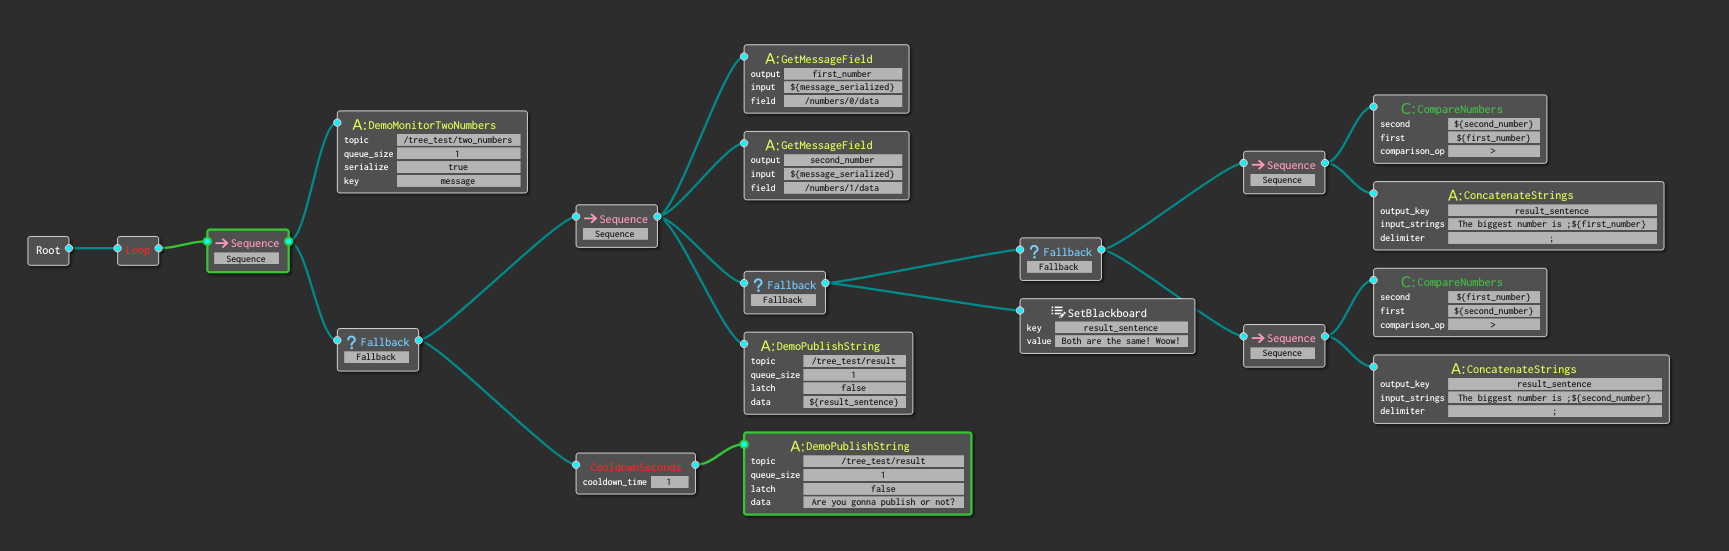
\includegraphics[width=\textwidth]{two_numbers_monitoring_1.png}
\caption{Real time tree monitoring with \textit{Groot}}
\label{figure:two-numbers-monitoring}
\end{figure}

The return status of each block will be represented by the color of the connection to its parent. Green means SUCCESS, red means FAILURE and a orange connection indicates that the block is returning RUNNING. Note that this feature is still a bit rough in the edges, so it may be difficult to know what's exactly going on sometimes.

\subsection{Adding Memory to your Trees}
\label{subsec:trees-memory}

The examples we have seen until now are said to be memoryless. This means that, every time a control node such as a sequence or a fallback was ticked, it ticked its children again from the beginning. This was not a problem in the previous trees, as all the nodes returned either SUCCESS or FAILURE immediately. There are, however, times when a node may return RUNNING as a status, either because its performing a task that takes a while to finish or because it's trying to control the timing/flow of the tree itself.

Consider the tree in figure \ref{figure:task-no-wait}. In each iteration, a new task is commanded and the processing is halted until it finishes. Let's assume also that the \textit{WaitForTaskToFinish} node returns RUNNING while the task is not finished. As it is right now, the tree is ill-formed and it will not work as expected. As soon as the wait node returns RUNNING, the sequence node will report back that to its parent. The loop will just tick the sequence again after that. However, as stated before, this sequence is memoryless, so in this new tick, it will start again the execution of its children from the beginning. This means a new task will be executed before the previous one is finished.

\begin{figure}[ht!]
\centering
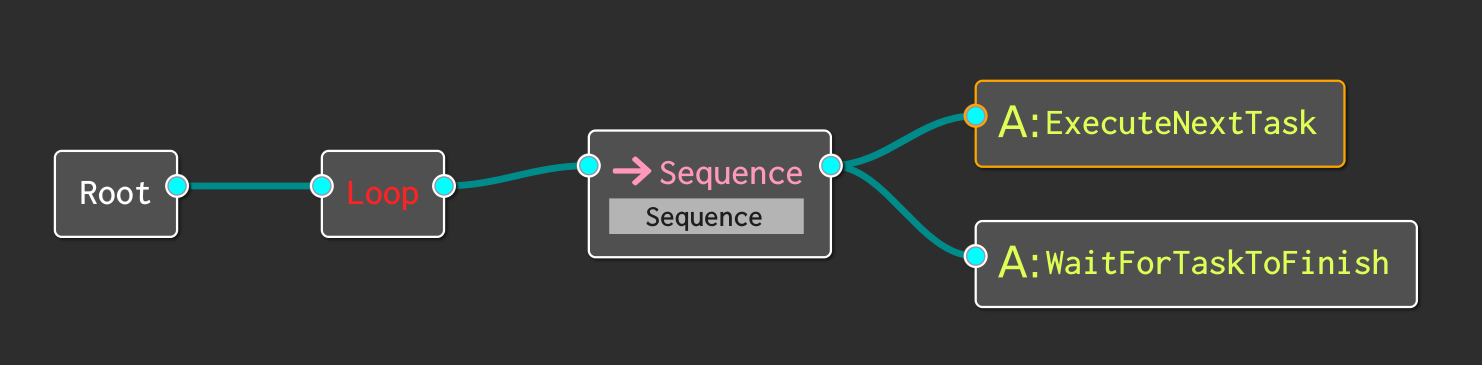
\includegraphics[width=\textwidth]{task_no_wait.png}
\caption{Ill-formed tree with no memory}
\label{figure:task-no-wait}
\end{figure}

This is obviously not what we want. Figure \ref{figure:wait-task} shows how to fix this. The vanilla sequence has been changed by its \textit{star} counterpart. All major control blocks have star versions with memory. Now, when the loop ticks again, the sequence will remember that one of its children returned RUNNING before, and it will tick it again to see if it has finished. This process will be repeated until it returns either SUCCESS or FAILURE.

\begin{figure}[ht!]
\centering
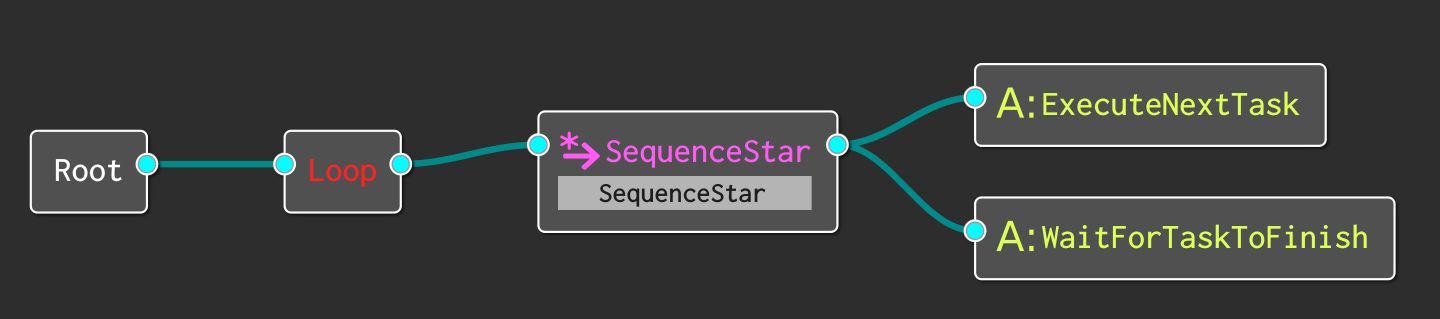
\includegraphics[width=\textwidth]{wait_task.png}
\caption{Correct tree using memory}
\label{figure:wait-task}
\end{figure}


After seeing this you may be tempted to add a control with memory every time you have a node that can return RUNNING somewhere under it. However, this can have unexpected results. Let's supposed now that we have to check the temperature levels of the system. If it ever gets above a threshold, missions should be aborted and the system should be turned off to ensure its integrity Figure \ref{figure:interruption-incorrect} depicts a possible implementation of this.

\begin{figure}[ht!]
\centering
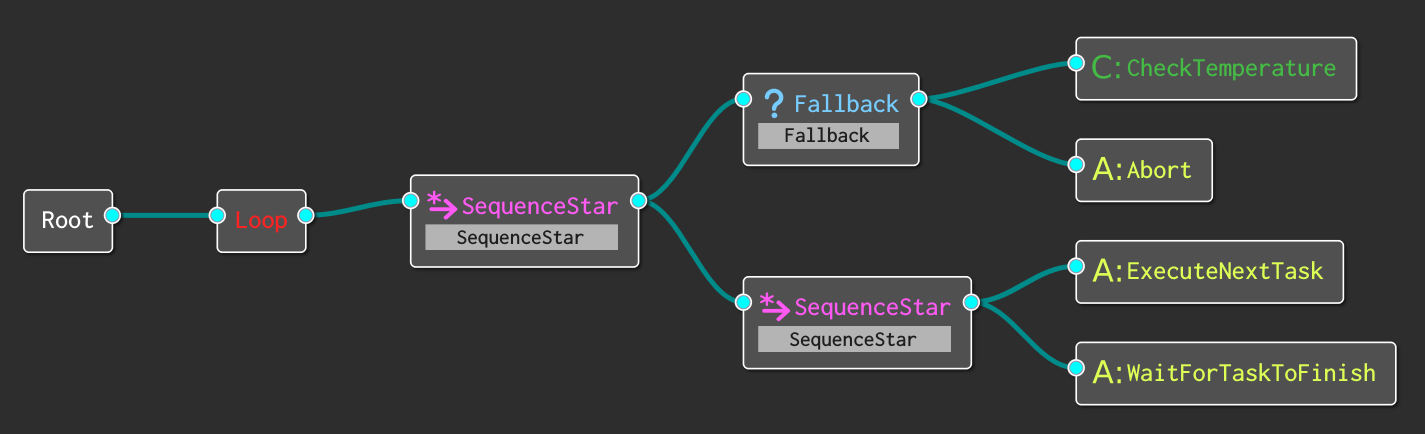
\includegraphics[width=\textwidth]{interruption_incorrect.png}
\caption{Tree lacking responsiveness due to bad memory placement}
\label{figure:interruption-incorrect}
\end{figure}

\textit{CheckTemperature} will return SUCCESS only if the system temperature is under the limits. If something goes wrong, it will return FAILURE, the fallback will switch to its second branch and the \textit{Abort} node will be executed.

Can you spot the issue here? The problem stems from the fact that both sequences have memory. The branch checking for the temperature will never be called while the system is waiting for a task to finish, as the outer sequence remembers one of its children returned RUNNING. Only after the task is finished and the external sequence is reseted the temperatures will be checked. Depending on how long the tasks are this could pose a problem or not.

The fix is rather simple, though. Simply switching the first sequence to its memoryless version does the trick. Figure \ref{figure:interruption-correct} shows the final result. Now, in every iteration the temperature will be checked first and after that the tasks branch will be executed, continuing from where it was left in the last iteration (either waiting for the current one to finish or commanding the next one).

\begin{figure}[ht!]
\centering
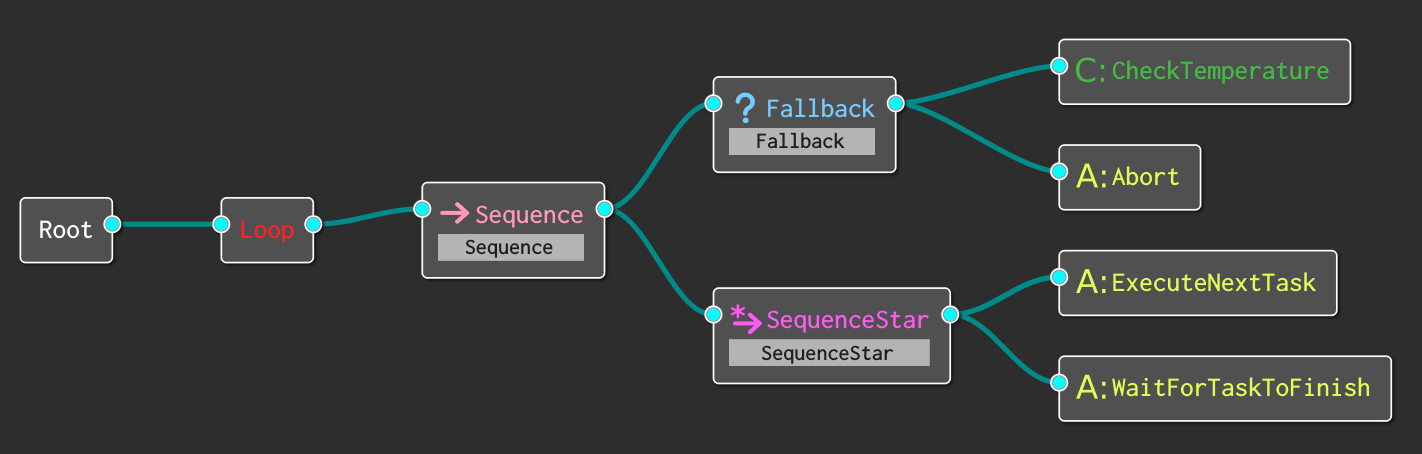
\includegraphics[width=\textwidth]{interruption_correct.png}
\caption{Proper multi-level memory management example}
\label{figure:interruption-correct}
\end{figure}

As seen in the above examples, special care should be taken when adding memory to a tree, as a bad placement of the \textit{star} control nodes can reduce the responsiveness of the behavior against important events dramatically. Placing blocks with memory correctly is the key to avoid this.

\subsection{Using Subtrees}
\label{subsec:monitoring-trees}

One of the major benefits of behavior trees is their high re-usability. Thanks to a simple interface (a node returns either SUCCESS, FAILURE or RUNNING), trees can be reused in other trees easily. This becomes even more important when the approach taken in the design is to use smaller general blocks along with introspection to execute basic operations on the input data, as shown in section \ref{subsec:trees-logic}. With this approach, big blocks containing chunks of code tailored to a specific task are substituted by subtrees made up of several simpler blocks.

Let's go back to the example of the two numbers presented in section \ref{subsec:trees-logic}. We would like to put all the logic to compare the two numbers inside its own subtree. This subtree would take as an input two numbers and will output a string containing the result of the comparison.

To create the new subtree right-click on the second \textit{fallback} node, just after the two \textit{GetMessageField} nodes and select the "\textit{Create Subtree Here}" option. And \textit{voil\`a}, you now have a valid subtree\footnote{In fact, this is currently the only way to create subtrees in \textit{Groot}. There's no method to create a new subtree from scratch, and trying to expand and empty subtree block will crash the application.}. All the blocks containing the comparison should have been substituted by a subtree block, as in figure \ref{figure:two_numbers_subtrees}. You can expand/collapse it in-situ, or you can inspect its contents by clicking on the tabs on top of the workspace.

\begin{figure}[ht!]
\centering
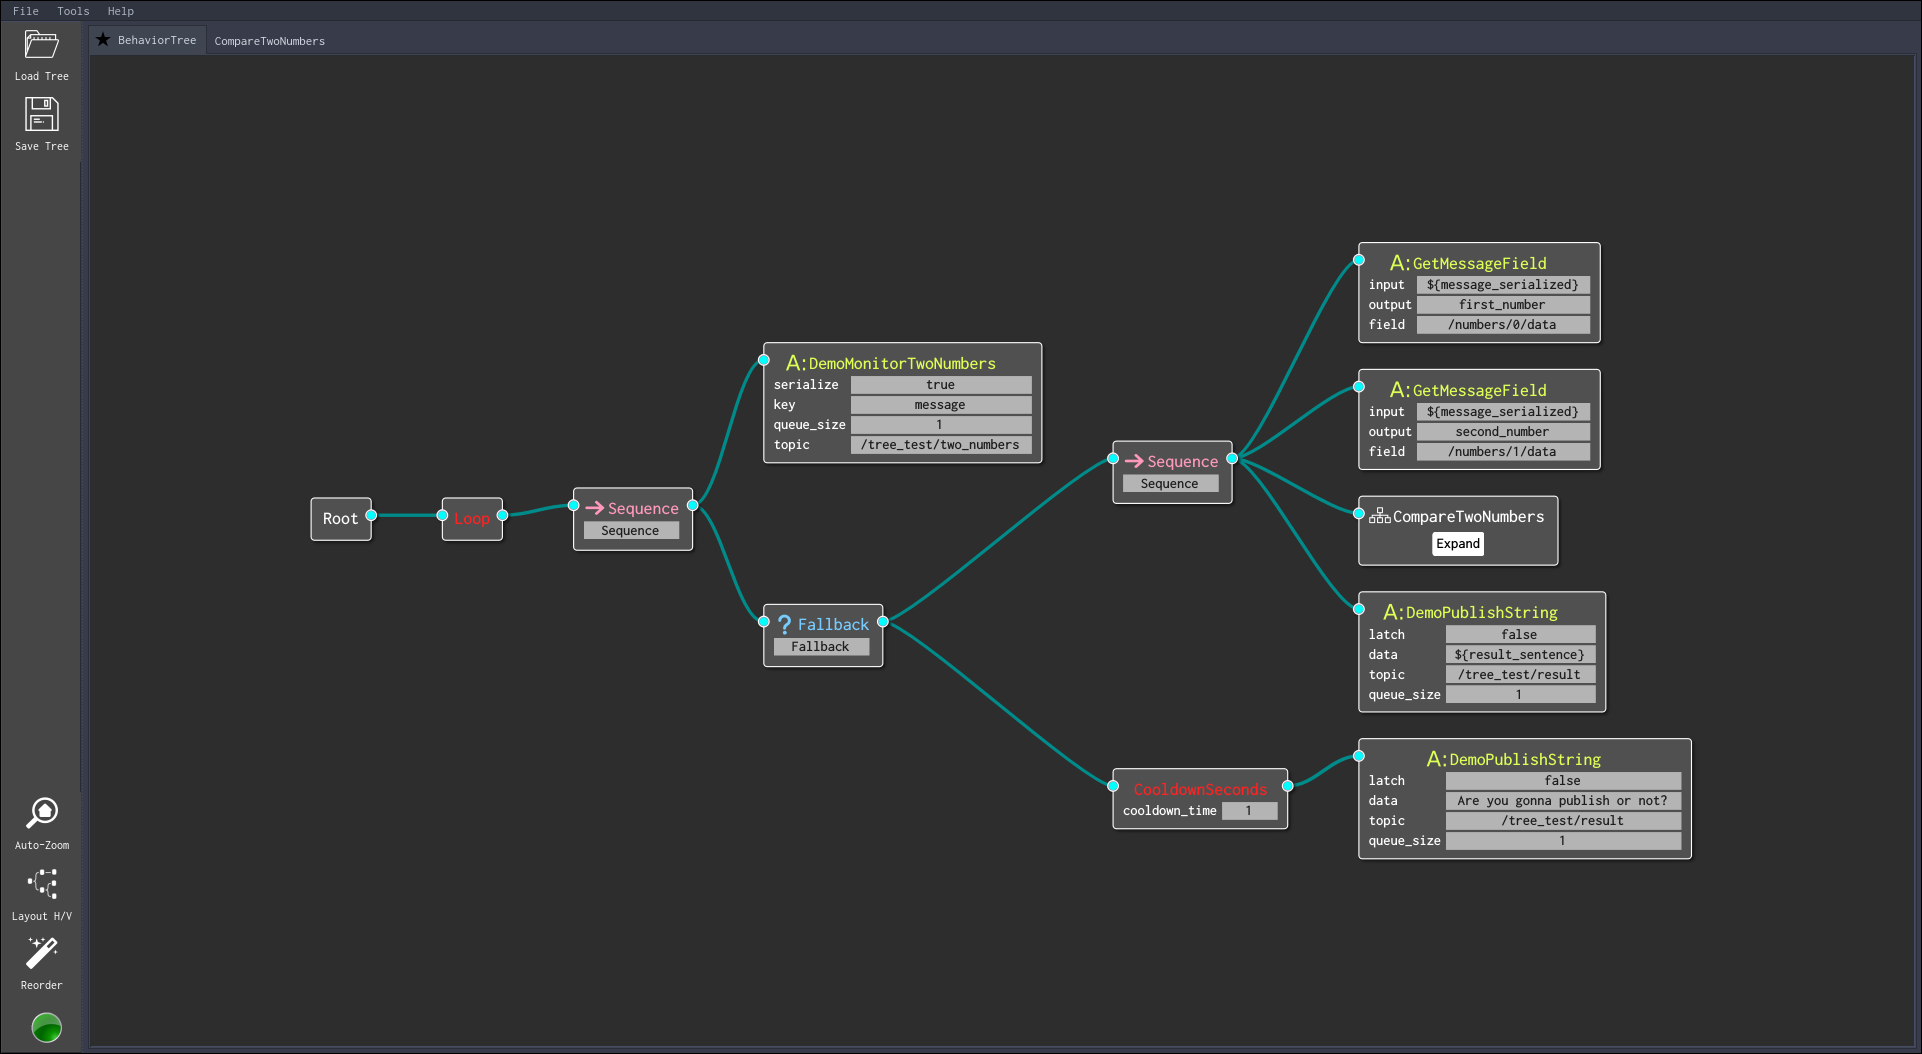
\includegraphics[width=\textwidth]{two_numbers_subtrees.png}
\caption{Tree containing a subtree}
\label{figure:two_numbers_subtrees}
\end{figure}

As stated before, the tree expects you to feed it two numbers in two different variables, and it gives you the result in another one. As it stands right now, there's no way to know what input and output ports a subtree has just by looking at the external block.

There are no distinctions made either between internal and external variables, so be careful when naming your variables. If you are not careful, you may end up overwriting internal variables of a subtree. Future versions of \textit{BehaviorTree.CPP} will account for this, and a port system similar to that of SMACH will be included to avoid name-clashing.

Remember also that all subtrees are available in the block list on the left, so you can instantiate them as many times as you want.

Let's take a look at the generated XML file to see the differences. Snippet \ref{listing:xml-subtree} shows the contents of the file, where the \textit{TreesNodesModel} section has been truncated for clarity. It's easy to see that the only addition to the file is a new \textit{BehaviorTree} section with the definition of the new tree. XML files should always have a root tree acting as the entry point. Line 1 declares the main tree to execute. Other trees defined in the file will be treated as subtrees.

\lstinputlisting[label={listing:xml-subtree},caption=Defining a subtree in a XML tree file]{snippets/two_numbers_subtrees.xml}


\subsection{Writing your own nodes}
\label{subsec:writing-nodes}

While manipulating ROS messages is fine and dandy, there are times you would like to write your own nodes (be it a leaf, control or decorator) to accomplish a given task or to add a new more general operation that was missing from the library. The online documentation is the main resource for this \cite{faconti_2019}.

Just some heads-up. Be careful when changing and reporting back result statuses. Your custom nodes shall never return IDLE. Control nodes will freak out and throw an exception, halting the whole tree. It's responsibility of the control nodes to set its children status back to IDLE, so you don't have to worry about that.

Also, avoid doing any sleep or performing any function that may take a while to finish. If you need to perform a long task, your node should return RUNNING immediately and run computations in parallel. Consider using techniques described in the online documentation such as coroutines or async actions.

\clearpage
\section{Nodes Reference}
\label{sec:behavior-trees-nodes}

Decoupling nodes code from the layout of the tree allow users to build trees using external graphical tools such as \textit{Groot}. However, it's sometimes difficult to understand exactly what a node does and when it should or shouldn't be used just by looking at its parameters in the GUI. You end up checking the code to fill in the gaps, which kind of defeats the point.

This section aims to present an exhaustive list of all the nodes currently available at \ac{SRL}. Nodes are classified by its nature or the system they are targeted at. Some nodes are available by default with \textit{BehaviorTree.CPP}, while others are more ROS-specific. There are also adaptations of nodes implemented by third-party well-known behavior trees frameworks, like the \textit{Unreal Engine Behavior Tree Editor} \cite{unreal_bt_reference}.

A summary describing what they do is provided, as well as input and output ports and expected variable types.


\subsection{Default nodes}
\label{subsec:default-nodes}

These nodes are pre-built with \textit{Groot} and \textit{BehaviorTree.CPP}. They are always available, even if no plugin has been imported.

\subsubsection{Decorator nodes}
\label{subsubsec:default-nodes-decorators}

\begin{longtable}[H]{ c M{0.35\textwidth} M{0.35\textwidth} }
\toprule
 \textbf{Block} &  \textbf{Description} &  \textbf{Ports} \\
 \midrule
	\begin{minipage}{.2\textwidth}
      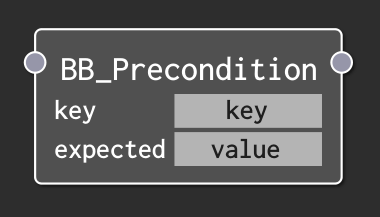
\includegraphics[width=\linewidth]{bb_precondition_node.png}
    \end{minipage} 
    & Returns SUCCESS if a given key exists in the blackboard and has an expected value.
    & \begin{minipage}{.35\textwidth}
    	   \textbf{key} Entry to check. \\
    	   \textbf{expected} Expected value (* for any).
    	   \end{minipage}
    \\ \midrule \\
 	\begin{minipage}{.2\textwidth}
      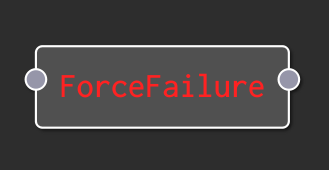
\includegraphics[width=\linewidth]{force_failure_node.png}
    \end{minipage}
    &  Returns FAILURE always, independently of its child's result.
    & No ports.
    \\ \midrule \\
    \begin{minipage}{.2\textwidth}
      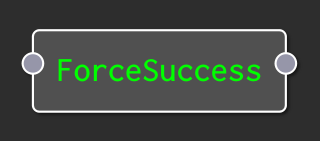
\includegraphics[width=\linewidth]{force_success_node.png}
    \end{minipage}
    &  Returns SUCCESS always, independently of its child's result.
    & No ports.
    \\ \midrule \\
    \begin{minipage}{.2\textwidth}
      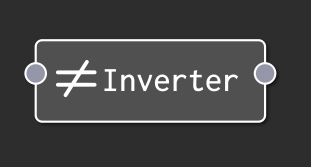
\includegraphics[width=\linewidth]{inverter_node.png}
    \end{minipage}
    &  Returns FAILURE if its child returns SUCCESS and SUCCESS otherwise (RUNNING status is not changed).
    & No ports.
    \\ \midrule \\
    \begin{minipage}{.2\textwidth}
      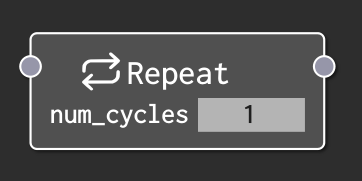
\includegraphics[width=\linewidth]{repeat_node.png}
    \end{minipage}
    &  Ticks its child a set number of times as long as it returns SUCCESS. Returns FAILURE and stops the cycle otherwise.
    & \begin{minipage}{.35\textwidth}
        \textbf{num_cycles} Maximum number of repetitions.
      \end{minipage}
    \\ \midrule \\
    \begin{minipage}{.2\textwidth}
      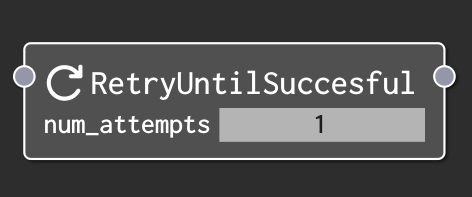
\includegraphics[width=\linewidth]{retry_node.png}
    \end{minipage}
    &  Keeps ticking its child until it returns SUCCESS.
    & \begin{minipage}{0.35\textwidth}
        \textbf{num_attemps} Maximum number of tries.
      \end{minipage}
    \\ \midrule \\
    \begin{minipage}{.2\textwidth}
      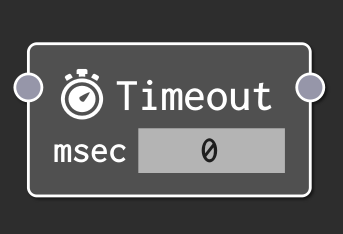
\includegraphics[width=\linewidth]{timeout_node.png}
    \end{minipage}
    &  Returns FAILURE and halts its child if it keeps returning RUNNING after a set time.
    & \begin{minipage}{0.35\textwidth}
      \textbf{msec} Timeout in milliseconds.
      \end{minipage}
	\\
 	\bottomrule
\caption{Default decorators nodes.}\label{table:default-nodes-decorators}
\end{longtable}

\subsubsection{Composite nodes}
\label{subsubsec:default-nodes-composite}

\begin{table}[H]
\begin{tabular}{ c M{0.35\textwidth} M{0.35\textwidth} }
\toprule
 \textbf{Block} &  \textbf{Description} &  \textbf{Ports} \\
 \midrule
	\begin{minipage}{.2\textwidth}
      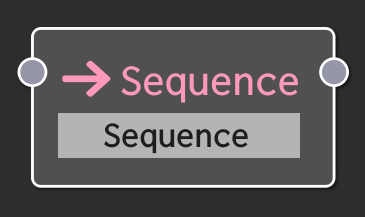
\includegraphics[width=\linewidth]{sequence_node.png}
    \end{minipage} 
    & Ticks its children in order. Returns SUCCESS if all of them return SUCCESS, RUNNING if any of them return it and it returns FAILURE and halts if any of them fails.
    & No ports.
    \\ \midrule \\
 	\begin{minipage}{.2\textwidth}
      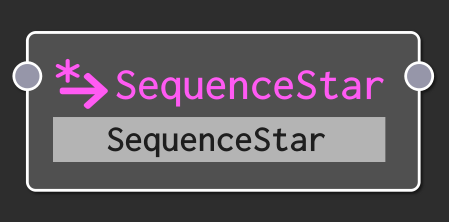
\includegraphics[width=\linewidth]{sequence_star_node.png}
    \end{minipage}
    &  Sequence block with memory.
    & No ports.
    \\ \midrule \\
    \begin{minipage}{.2\textwidth}
      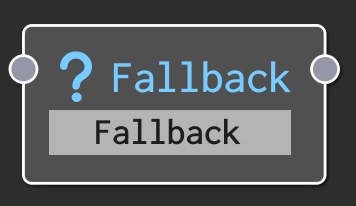
\includegraphics[width=\linewidth]{fallback_node.png}
    \end{minipage}
    &  Returns SUCCESS and stops when one of its children returns SUCCESS, ticks the next one otherwise.
    & No ports.
    \\ \midrule \\
    \begin{minipage}{.2\textwidth}
      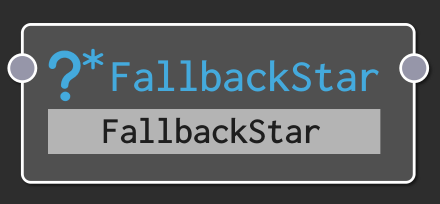
\includegraphics[width=\linewidth]{fallback_star_node.png}
    \end{minipage}
    &  Returns SUCCESS always independently of its child's result.
    & No ports.
    \\ \midrule \\
    \begin{minipage}{.2\textwidth}
      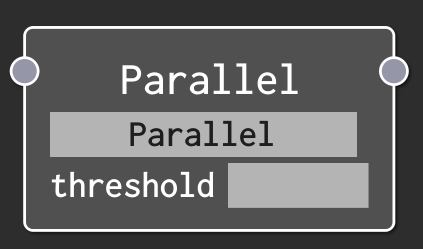
\includegraphics[width=\linewidth]{parallel_node.png}
    \end{minipage}
    &  Ticks all its children at the same time. Returns FAILURE and halts the process if a set number of children returns it.
    &\begin{minipage}{0.35\textwidth}
      	\textbf{threshold} Maximum number of children that can fail.
     \end{minipage}
	\\
 	\bottomrule
\end{tabular}
\caption{Default composite nodes.}\label{table:default-nodes-composite}
\end{table}

\subsubsection{Leaf nodes}
\label{subsubsec:default-nodes-leaf}

\begin{table}[H]
\begin{tabular}{ c M{0.35\textwidth} M{0.35\textwidth} }
\toprule
 \textbf{Block} &  \textbf{Description} &  \textbf{Ports} \\
 \midrule
	\begin{minipage}{.2\textwidth}
      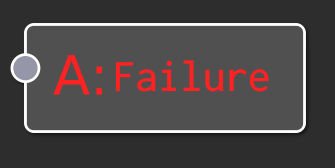
\includegraphics[width=\linewidth]{always_failure_node.png}
    \end{minipage} 
    & Returns FAILURE always.
    & No ports.
    \\ \midrule \\
 	\begin{minipage}{.2\textwidth}
      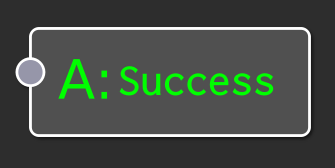
\includegraphics[width=\linewidth]{always_success_node.png}
    \end{minipage}
    &  Returns SUCCESS always.
    & No ports.
    \\ \midrule \\
    \begin{minipage}{.2\textwidth}
      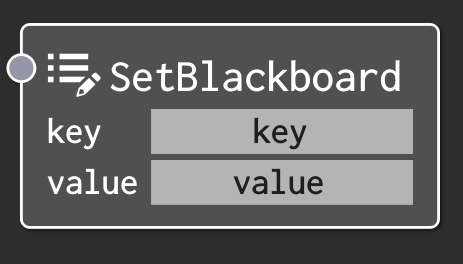
\includegraphics[width=\linewidth]{set_blackboard_node.png}
    \end{minipage}
    &  Inserts a new entry in the blackboard.
    & \begin{minipage}{0.35\textwidth}
        \textbf{key} Name of the new entry.
        \textbf{value} Value of the new entry.
     \end{minipage}
	\\
 	\bottomrule
\end{tabular}
\caption{Default leaf nodes.}\label{table:default-nodes-leaf}
\end{table}

\subsection{Introspection nodes}
\label{subsec:introspection-nodes}

These nodes can be found in the \textit{behavior_tree_ros} package plugin. They offer message-agnostic operations and operates on serialized ROS messages.

\subsubsection{Decorator nodes}
\label{subsubsec:introspection-nodes-decorators}

\begin{table}[H]
\begin{tabular}{ c M{0.35\textwidth} M{0.35\textwidth} }
\toprule
 \textbf{Block} &  \textbf{Description} &  \textbf{Ports} \\
 \midrule
	\begin{minipage}{.2\textwidth}
      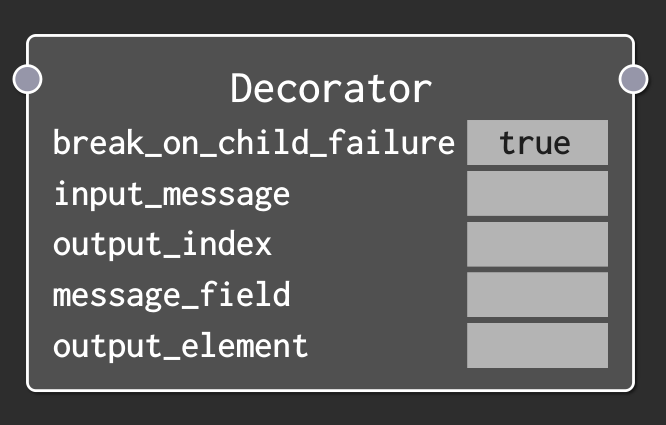
\includegraphics[width=\linewidth]{for_each_loop_node.png}
    \end{minipage} 
    & Node implementing a \textit{forEach} loop over a sequence. For each entry in the input sequence it will tick its child.
    & \begin{minipage}{0.35\textwidth}
       	\textbf{break_on_child_failure} If true, it will return FAILURE and halt the loop if its child returns FAILURE. \\
        \textbf{input_message} Serialized ROS message input. \\
        \textbf{message_field} JSON pointer to the sequence in the ROS message to iterate through. \\
        \textbf{output_index} Optional variable name used to save the current sequence entry index. \\
        \textbf{output_element} Optional variable name used to save the current sequence entry element. \\
      \end{minipage}
	\\
 	\bottomrule
\end{tabular}
\caption{Introspection decorator nodes.}\label{table:introspection-nodes-decorator}
\end{table}

\subsubsection{Leaf nodes}
\label{subsubsec:introspection-nodes-leaf}

\begin{table}[H]
\begin{tabular}{ c M{0.35\textwidth} M{0.35\textwidth} }
\toprule
 \textbf{Block} &  \textbf{Description} &  \textbf{Ports} \\
 \midrule
	\begin{minipage}{.2\textwidth}
      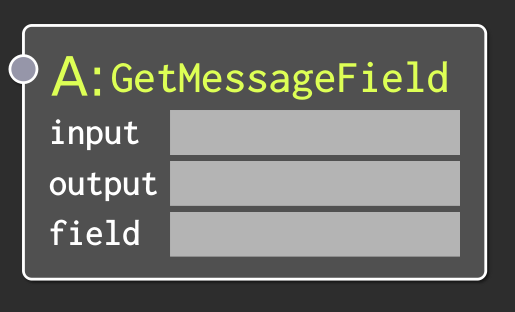
\includegraphics[width=\linewidth]{get_message_field_node.png}
    \end{minipage} 
    & Extracts a field from a serialized ROS message. Type safety ensured.
    & \begin{minipage}{0.35\textwidth}
        \textbf{input} Serialized ROS message input. \\
        \textbf{field} JSON pointer to the field to extract. \\
        \textbf{output} Output variable name. \\
      \end{minipage}
    \\ \midrule \\
 	\begin{minipage}{.2\textwidth}
      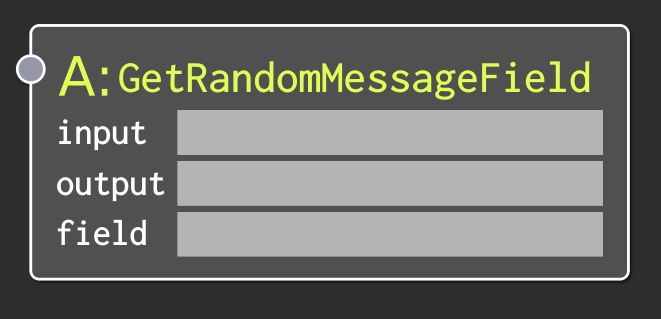
\includegraphics[width=\linewidth]{get_random_message_field_node.png}
    \end{minipage}
    & Extracts a random entry from a sequence.
    & \begin{minipage}{0.35\textwidth}
        \textbf{input} Serialized ROS message input. \\
        \textbf{field} JSON pointer to the sequence. \\
        \textbf{output} Output variable name.
      \end{minipage}
    \\ \midrule \\
    \begin{minipage}{.2\textwidth}
      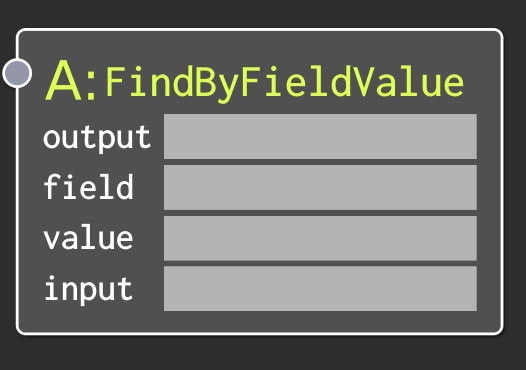
\includegraphics[width=\linewidth]{find_by_field_value_node.png}
    \end{minipage}
    &  Finds an entry in a sequence with a given value.
    & \begin{minipage}{0.35\textwidth}
        \textbf{input} Serialized ROS message input. \\
        \textbf{field} JSON pointer to the sequence. \\
        \textbf{output} Output variable name. \\
        \textbf{value} Value to search.
      \end{minipage}
	\\
 	\bottomrule
\end{tabular}
\caption{Introspection leaf nodes.}\label{table:introspection-nodes-leaf}
\end{table}

\subsection{TF nodes}
\label{subsec:tf-nodes}

Some TF-related nodes are available in the \textit{behavior_tree_extensions} package plugin.

\subsubsection{Leaf nodes}
\label{subsubsec:tf-nodes-leaf}

\begin{longtable}[H]{ M{0.2\textwidth} M{0.35\textwidth} M{0.35\textwidth} }
\toprule
 \textbf{Block} &  \textbf{Description} &  \textbf{Ports} \\
 \midrule
	\begin{minipage}{.2\textwidth}
      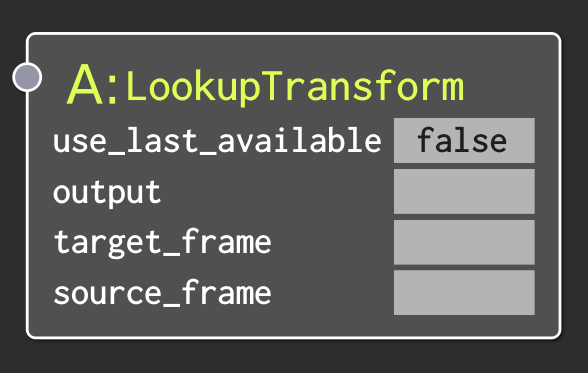
\includegraphics[width=\linewidth]{look_up_transform_node.png}
    \end{minipage} 
    & Queries the TF system for a transform between two frames. The resulting TF message will not be serialized.
    & \begin{minipage}{0.35\textwidth}
        \textbf{use_last_available} If true, use last transform available. Search using the current system time otherwise. \\
        \textbf{output} Variable used to save the result. \\
        \textbf{target_frame} Target TF frame. \\
        \textbf{source_frame} Source TF frame.
      \end{minipage}
    \\ \midrule \\
 	\begin{minipage}{.2\textwidth}
      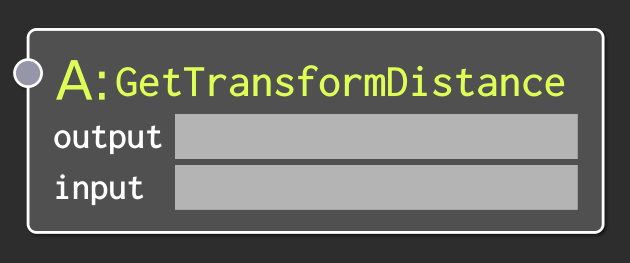
\includegraphics[width=\linewidth]{get_transform_distance_node.png}
    \end{minipage}
    &  Computes the 3D distance of a TF transform.
    & \begin{minipage}{0.35\textwidth}
        \textbf{input} Input TF transform message (not serialized). \\
        \textbf{output} Variable used to save the result.
      \end{minipage}
    \\ \midrule \\
    \begin{minipage}{.2\textwidth}
      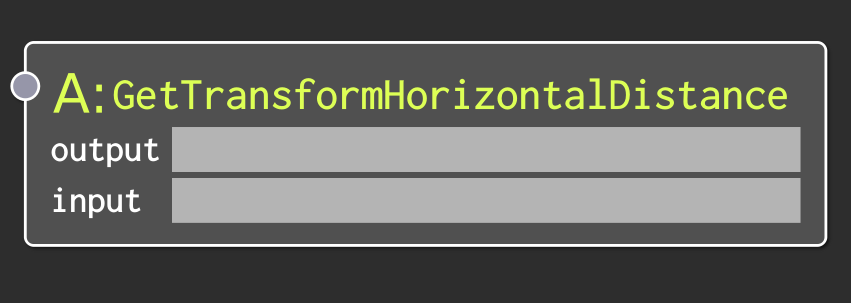
\includegraphics[width=\linewidth]{get_transform_horizontal_distance_node.png}
    \end{minipage}
    &  Computes the 2D distance (distance over the X-Y plane) of a TF transform.
    & \begin{minipage}{0.35\textwidth}
        \textbf{input} Input TF transform message (not serialized). \\
        \textbf{output} Variable used to save the result.
      \end{minipage}
	\\
 	\bottomrule
\caption{TF leaf nodes.}\label{table:tf-nodes-leaf}
\end{longtable}

\subsection{Haru nodes}
\label{subsec:haru-nodes}

Nodes specific to Haru. Available in the \textit{behavior_tree_haru} package plugin. Ports related to the publisher (topic, latch and queue_size) or to service clients (service name) are not included in the table.

\subsubsection{Leaf nodes}
\label{subsubsec:haru-nodes-leaf}

\begin{longtable}[H] { c M{0.35\textwidth} M{0.35\textwidth} }
\toprule
 \textbf{Block} &  \textbf{Description} &  \textbf{Ports} \\
 \midrule
	\begin{minipage}{.2\textwidth}
      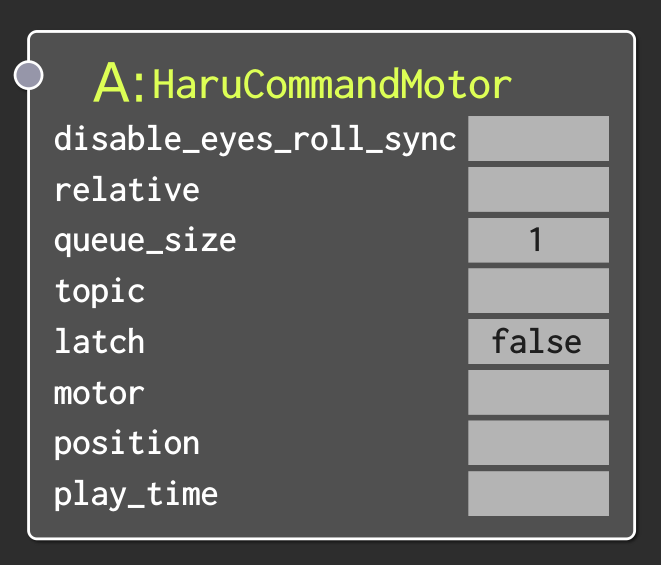
\includegraphics[width=\linewidth]{haru_command_motor_node.png}
    \end{minipage} 
    & Publishes a \textit{MotorCommand} message.
    & \begin{minipage}{0.35\textwidth}
        \textbf{disable_eyes_roll_sync} Disable LCD eyes video and roll sync. \\
        \textbf{relative} Set command relative to current position. \\
        \textbf{motor} Motor ID [0-4]. \\
        \textbf{position} Target position in radians. \\
        \textbf{play_time} Movement duration [0-250].
      \end{minipage}
    \\ \midrule \\
 	\begin{minipage}{.2\textwidth}
      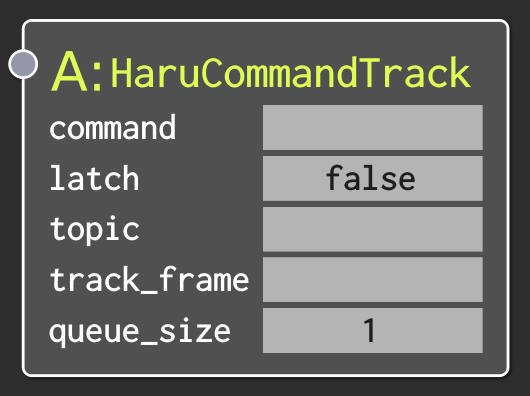
\includegraphics[width=\linewidth]{haru_command_track_node.png}
    \end{minipage}
    &  Publishes a \textit{TrackCommand} message.
    & \begin{minipage}{0.35\textwidth}
        \textbf{command} Command ID: 0 start tracking and 1 to stop. \\
        \textbf{track_frame} TF frame to track.
      \end{minipage}
    \\ \midrule \\
    \begin{minipage}{.2\textwidth}
      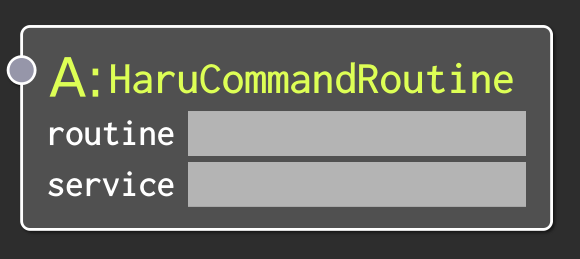
\includegraphics[width=\linewidth]{haru_command_routine_node.png}
    \end{minipage}
    &  Commands a routine using the \textit{idmind_tabletop/execute_routine} service.
    & \begin{minipage}{0.35\textwidth}
        \textbf{routine} Routine ID.
      \end{minipage}
    \\ \midrule \\
 	\begin{minipage}{.2\textwidth}
      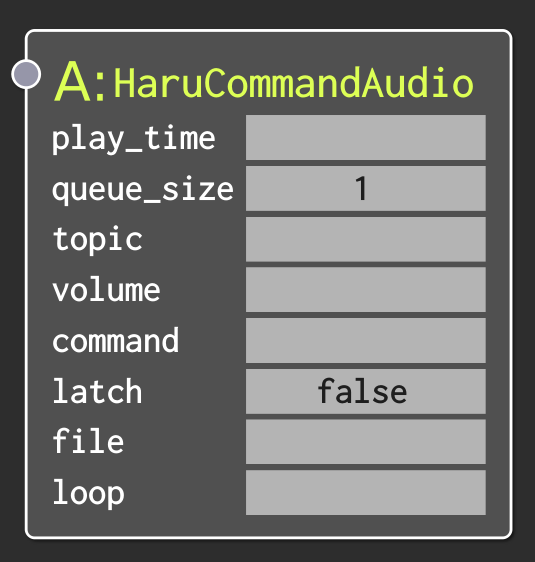
\includegraphics[width=\linewidth]{haru_command_audio_node.png}
    \end{minipage}
    &  Publishes an \textit{AudioCommand} message.
    & \begin{minipage}{0.35\textwidth}
        \textbf{command} Command ID: 0 start playing the file and 1 to stop. \\
        \textbf{file} Audio wave file to play. \\
        \textbf{volume} Volume level [0.0-1.0]. \\
        \textbf{loop} Loop file. \\
        \textbf{play_time} Duration in milliseconds the file should be played (0 means the whole file).
      \end{minipage}
    \\ \midrule \\
 	\begin{minipage}{.2\textwidth}
      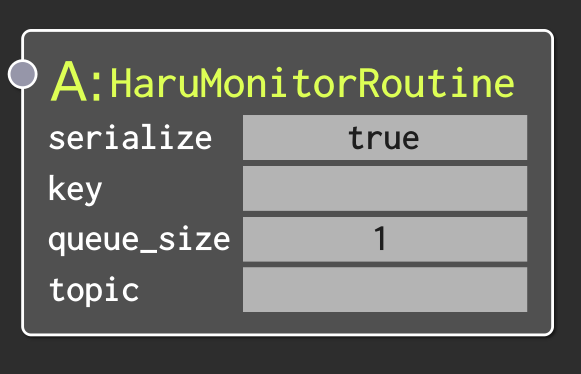
\includegraphics[width=\linewidth]{haru_monitor_routine_node.png}
    \end{minipage}
    &  Subscribes to a \textit{RoutineStatus} message type topic.
    & Subscriber's default ports.
    \\ \midrule \\
 	\begin{minipage}{.2\textwidth}
      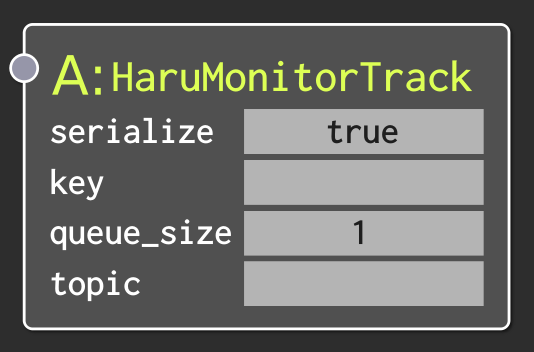
\includegraphics[width=\linewidth]{haru_monitor_track_node.png}
    \end{minipage}
    &  Subscribes to a \textit{TrackStatus} message type topic.
    & Subscriber's default ports.
	\\
 	\bottomrule
\caption{Haru leaf nodes.}\label{table:haru-nodes-leaf}
\end{longtable}

\subsection{Strawberry nodes}
\label{subsec:strawberry-nodes}

Strawberry-related nodes. Available in the \textit{behavior_tree_strawberry} package plugin. Ports related to the publisher (topic, latch and queue_size) or to service clients (service name) are not included in the table.

\subsubsection{Leaf nodes}
\label{subsubsec:strawberry-nodes-leaf}

\begin{table}[H]
\begin{tabular}{ M{0.2\textwidth} M{0.35\textwidth} M{0.35\textwidth} }
\toprule
 \textbf{Block} &  \textbf{Description} &  \textbf{Ports} \\
 \midrule
	\begin{minipage}{.2\textwidth}
      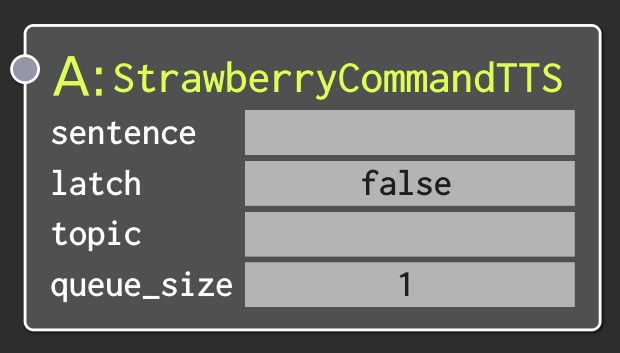
\includegraphics[width=\linewidth]{strawberry_command_tts_node.png}
    \end{minipage} 
    & Publishes a \textit{TTSCommand} message.
    & \begin{minipage}{0.35\textwidth}
        \textbf{sentence} String containing the sentence to send to the TTS system.
      \end{minipage}
    \\ \midrule \\
 	\begin{minipage}{.2\textwidth}
      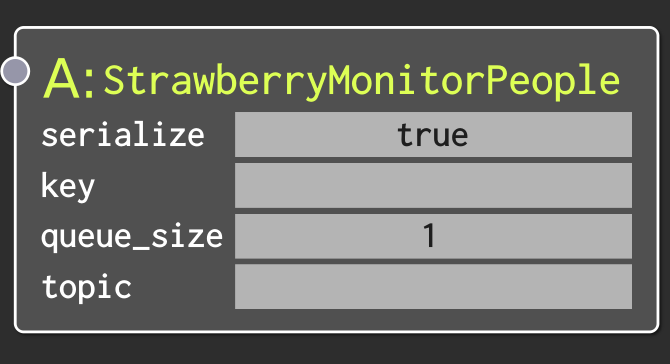
\includegraphics[width=\linewidth]{strawberry_monitor_people_node.png}
    \end{minipage}
    &  Subscribes to a \textit{People} message type topic.
    & Subscriber's default ports.
	\\
 	\bottomrule
\end{tabular}
\caption{Strawberry leaf nodes.}\label{table:strawberry-nodes-leaf}
\end{table}

\subsection{Misc nodes}
\label{subsec:misc-nodes}

This section contains nodes that cannot really be put into any other category, such as waits, loops or comparisons. They are basic basic building blocks that are used in pretty much any behavior tree. Keep in mind that they do not rely in ROS messages introspection.

\subsubsection{Decorator nodes}
\label{subsubsec:extension-nodes-decorators}

\begin{table}[H]
\begin{tabular}{ c M{0.35\textwidth} M{0.35\textwidth} }
\toprule
 \textbf{Block} &  \textbf{Description} &  \textbf{Ports} \\
 \midrule
	\begin{minipage}{.2\textwidth}
      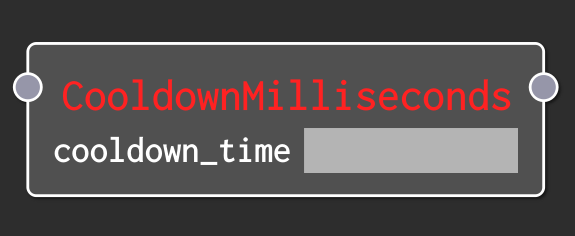
\includegraphics[width=\linewidth]{cooldown_node.png}
    \end{minipage} 
    & Sets a maximum tick rate for its child. After being ticked, it will keep returning its child last return value until the cooldown time has passed.
    & \begin{minipage}{0.35\textwidth}
        \textbf{cooldown_time} Cooldown time.
      \end{minipage}
    \\ \midrule \\
 	\begin{minipage}{.2\textwidth}
      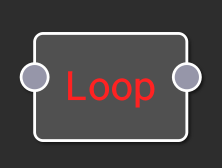
\includegraphics[width=\linewidth]{loop_node.png}
    \end{minipage}
    &  Keeps ticking its child independently of its return value.
    & No ports.
    \\ \midrule \\
    \begin{minipage}{.2\textwidth}
      
\includegraphics[width=\linewidth]{while_success_node.png}
    \end{minipage}
    &  Keeps ticking its child as long as it returns SUCCESS.
    & No ports.
	\\
 	\bottomrule
\end{tabular}
\caption{Misc decorator nodes.}\label{table:misc-nodes-decorator}
\end{table}

\subsubsection{Leaf nodes}
\label{subsubsec:misc-nodes-leaf}

\begin{longtable}[!htp]{ c M{0.35\textwidth} M{0.35\textwidth} }
\toprule
 \textbf{Block} &  \textbf{Description} &  \textbf{Ports} \\
 \midrule
	\begin{minipage}{.2\textwidth}
      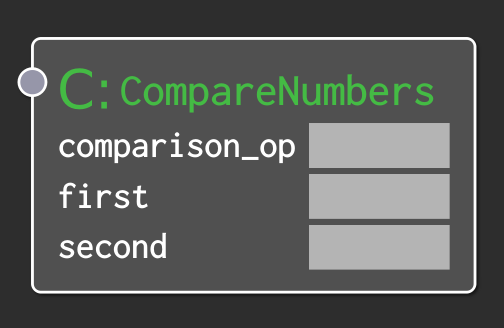
\includegraphics[width=\linewidth]{compare_numbers_node.png}
    \end{minipage} 
    & Compare two numbers (integer or float) using the comparison operator set by the user. Returns SUCCESS if the comparison is true or FAILURE otherwise.
    & \begin{minipage}{0.35\textwidth}
        \textbf{comparison_op} Comparison operator. Valid values are: ==, !=, <, <=, > and >=. \\
        \textbf{first} Left operand. \\
        \textbf{second} Right operand.
      \end{minipage}
    \\ \midrule \\
 	\begin{minipage}{.2\textwidth}
      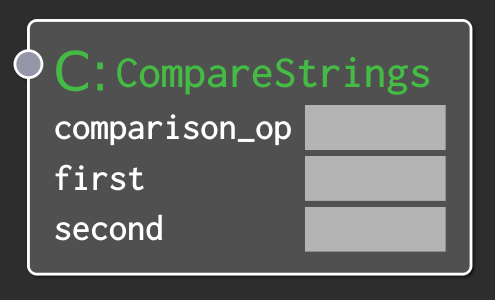
\includegraphics[width=\linewidth]{compare_strings_node.png}
    \end{minipage}
    & Comparison block (strings version).
    & Same as \textit{CompareNumbers} node.
    \\ \midrule \\
    \begin{minipage}{.2\textwidth}
      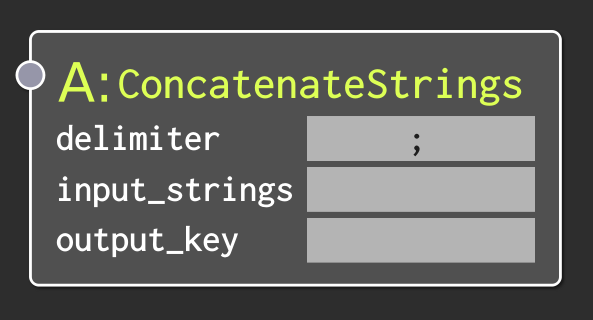
\includegraphics[width=\linewidth]{concatenate_strings_node.png}
    \end{minipage}
    &  Concatenate the strings in the input sequence.
    & \begin{minipage}{0.35\textwidth}
        \textbf{delimiter} Input sequence entries delimiter (defaults to ';'). \\
        \textbf{input_strings} Sequence containing the strings to concatenate. \\
        \textbf{output_key} Output variable.
      \end{minipage}
    \\ \midrule \\
 	\begin{minipage}{.2\textwidth}
      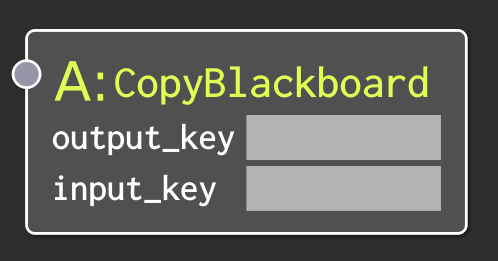
\includegraphics[width=\linewidth]{copy_blackboard_node.png}
    \end{minipage}
    &  Copies the contents of one blackboard's entry to another.
    & \begin{minipage}{0.35\textwidth}
        \textbf{input_key} Input variable. \\
        \textbf{output_key} Output variable.
      \end{minipage}
    \\ \midrule \\
 	\begin{minipage}{.2\textwidth}
      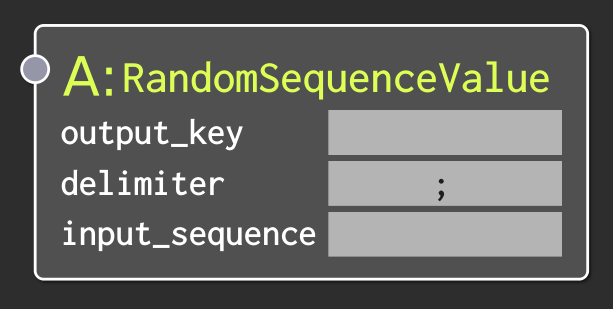
\includegraphics[width=\linewidth]{random_sequence_value_node.png}
    \end{minipage}
    &  Gets a random entry from an input sequence.
    & \begin{minipage}{0.35\textwidth}
        \textbf{delimiter} Input sequence entries delimiter (defaults to ';'). \\
        \textbf{input_sequncee} Input sequence. \\
        \textbf{output_key} Output variable.
      \end{minipage}
    \\ \midrule \\
 	\begin{minipage}{.2\textwidth}
      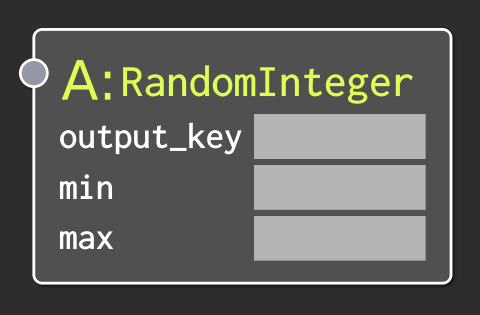
\includegraphics[width=\linewidth]{random_integer_node.png}
    \end{minipage}
    & Returns a random integer in the range [min,max].
    & \begin{minipage}{0.35\textwidth}
        \textbf{min} Range minimum value. \\
        \textbf{max} Range maxximum value. \\
        \textbf{output_key} Output variable.
      \end{minipage}
    \\ \midrule \\
 	\begin{minipage}{.2\textwidth}
      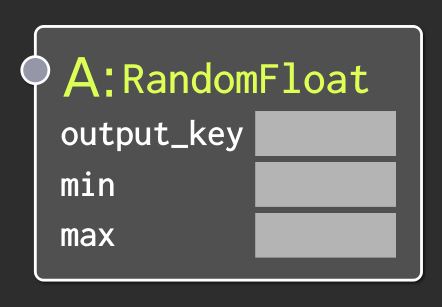
\includegraphics[width=\linewidth]{random_float_node.png}
    \end{minipage}
    &  Returns a random integer in the range [min,max].
    & Same as \textit{RandomInteger} node.
    \\ \midrule \\
 	\begin{minipage}{.2\textwidth}
      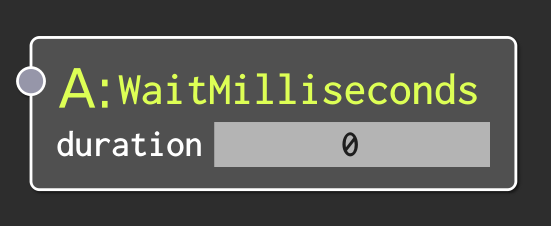
\includegraphics[width=\linewidth]{wait_node.png}
    \end{minipage}
    &  Returns RUNNING for a set amount of time. Returns SUCCESS when it's done.
    & \begin{minipage}{0.35\textwidth}
        \textbf{duration} Wait time in milliseconds.
      \end{minipage}
	\\
 	\bottomrule
\caption{Misc leaf nodes.}\label{table:misc-nodes-leaf}
\end{longtable}

\clearpage
\section{Behavior Trees Cookbook}
\label{sec:behavior-trees-cookbook}

Even though trees are rather simple in concept, thinking in terms of them not so much. There might be times you hit a dead wall trying to express some logic, unable to find the right connection between decorator, control and leaf nodes that gives you the logic flow you need.

This section aims to mitigate that, providing some common general structures and tricks you can use in your own trees. This is a constant work-in-progress. The more we work with trees, the more it will grow with good practices and know-how.

\subsection{While Loops}
\label{subsec:cookbook-while-loop}

While loops are one of the basics way to control the flow of a program. There are times you may have the need to express this same concept of "\textit{while X do Y}" in your trees. Let's use a real example to illustrate how to achieve this.

Haru, the social robot in the lab offers several ways to interact with it, one of them being via physical gestures. When the person currently engaged (that is, being tracked) does a gesture, it should do some animation as a response. However, for security reasons, tracking should be halted while the animation is playing. Basically we have a "\textit{while the tracked person is present do ...}" structure.

There are mainly two ways to express this. Figure \ref{figure:while_loop_method_1} shows a first alternative. Here we are exploiting the fact that memory is always local to a block (this was explained in section \ref{subsec:trees-memory}). The condition is put in the first branch and the loop body in the second. The first sequence has no memory, so the \textit{IsTrackedPersonPresent} condition will always be checked first. After that, the second branch, containing the gesture detection and animation response is executed from where it was left in the last iteration.

\textit{Retry} and \textit{Timeout} blocks are added at the beginning to get out of the loop if the person does nothing during a preset amount of time.

\begin{figure}[ht!]
\centering
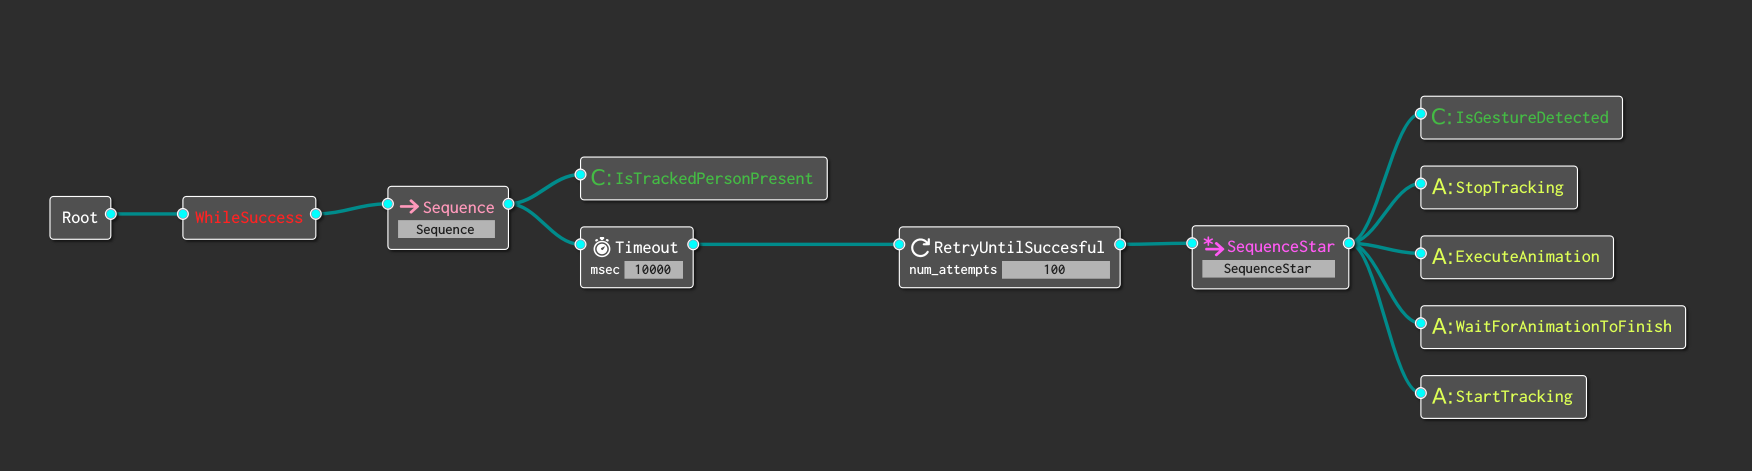
\includegraphics[width=\textwidth]{while_loop_method_1.png}
\caption{Implementing a while loop in a tree}
\label{figure:while_loop_method_1}
\end{figure}

The second method may be a bit more easy to understand visually. Figure \ref{figure:while_loop_method_2} shows it. Here, the condition and the loop body are split in the two branches of the initial \textit{Parallel} block. This block will tick alternatively its children. The parameter \textit{threshold} is the number of branches that have to return SUCCESS for the whole parallel block to report SUCCESS back to its parent.

In other words, with a threshold of 2 and 2 connected branches, we have that 0 branches can return FAILURE before all processing is halted. If any of the two branches fails we get out of the loop. The two \textit{WhileSuccess} in each branch ensure that we keep looping while the conditions are true.

Both versions are equivalent, as there's no overhead to the \textit{Parallel} node.

\begin{figure}[ht!]
\centering
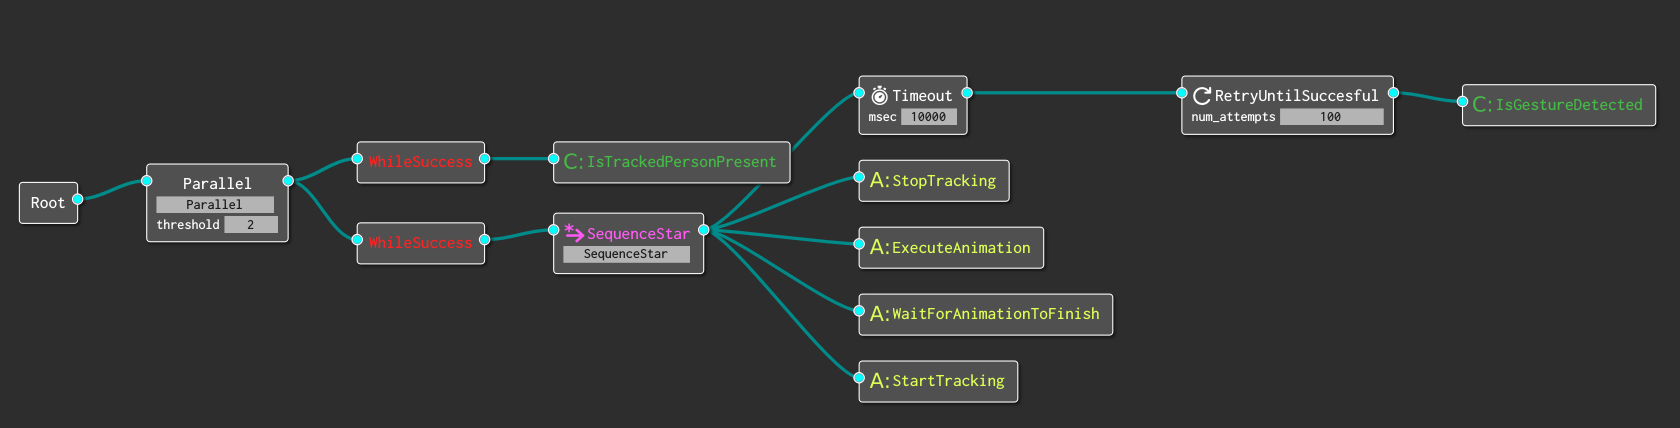
\includegraphics[width=\textwidth]{while_loop_method_2.png}
\caption{Alternative way to implement a while loop in a tree}
\label{figure:while_loop_method_2}
\end{figure}


\clearpage
\section{Conclusions}
\label{sec:conclusions}

Behavior trees present the flexibility, modularity and re-usability necessary to build a general behavior framework. This would speed up development times and unify the way behavior and decision-making in general is built in \ac{SRL}. By generalizing ROS structures, it's possible to develop message-agnostic nodes containing the most basic operations, thus avoiding ad-hoc applications tailored to the specific needs of a given project.

\clearpage
\addcontentsline{toc}{section}{References}
\bibliographystyle{IEEEtran}
\bibliography{bibliography}

\newpage
\appendix

\section{ROS Messages Introspection}
\label{annex:introspection}

As it was discussed in section \ref{subsec:trees-logic}, \textit{behavior_tree_ros} package offers publishers and subscribers leaf nodes that can manipulate ROS messages without the need to write any additional line of code. This annexe contains a technical description on how this works, as well limitations and workarounds.

ROS code generators include in the messages generated static info about their own types and structure that can be later queried at compile time. This info comes in the form of a string describing the field messages and types in order. This can be parsed to achieve a pseudo-introspection\footnote{You actually need to get to know somehow what's the type of the message. Hence the need to state it in the plugin.} on runtime for any given message.

\textit{behavior_tree_ros} relies on \textit{ros_type_introspection} package to do the parsing of this static info. Later you can feed it a raw buffer containing a non-deserialized message, and it will construct a general tree (not a behavior tree) with the same structure as the original message, field names, types and their values.

This tree is not too user friendly, though. Figure \ref{figure:two-numbers-tree} shows the tree representation of the \textit{TwoNumbers} message defined back in section \ref{subsec:trees-logic}. Only the nodes' names are represented. Internally, each node contains an identifier of its type and its value.

\begin{figure}[ht!]
\centering
\begin{forest}
  forked edges,
  [/behavior_tree_demo/TwoNumbers
    [/header
    		[/seq]
    		[/stamp
    			[/data]
    		]
    		[/frame_id]
    ]
    [/numbers
      [.0
      	[/data]
      ]
      [.1,
      	[/data]
      ]
    ]
  ]
\end{forest}
\caption{Tree representation of \textit{TwoNumbers} message}
\label{figure:two-numbers-tree}
\end{figure}

\textit{ros_type_introspection} offers a \textit{flattened} version of the tree as well. A hierarchical structure is said to be flattened when it has only one level containing all the leaf nodes. Each leaf node is qualified by its full name, generated as the concatenation of all the nodes' identifiers that have to be transversed starting from the root to reach it. Figure \ref{figure:two-numbers-tree-flatten} shows the flattened version of the tree, where actual values have been omitted.

\begin{figure}[ht!]
\centering
\begin{lstlisting}[language=json, basicstyle=\small]
{
  "behavior_tree_demo/TwoNumbers/header/seq": ,
  "behavior_tree_demo/TwoNumbers/header/stamp/data": ,
  "behavior_tree_demo/TwoNumbers/header/frame_id": ,
  "behavior_tree_demo/TwoNumbers/numbers.0/data": ,
  "behavior_tree_demo/TwoNumbers/numbers.1/data":
}
\end{lstlisting}
\caption{Flatten tree representation of \textit{TwoNumbers} message}
\label{figure:two-numbers-tree-flatten}
\end{figure}

This structure is nearly identical to a flattened JSON, where its keys are JSON pointers as defined in \href{https://tools.ietf.org/html/rfc6901}{RFC 6901}. The only difference being that arrays indexes are preceded by a point instead of a slash. Replacing them by the correct delimiter enable us to instantiate a proper JSON object. Figure \ref{figure:two-numbers-tree-json} shows the result.

\begin{figure}[ht!]
\centering
\begin{lstlisting}[language=json, basicstyle=\small]
{
  "header": 
  {
  	"seq": ...,
  	"stamp": { "data": ... },
  	"frame_id": ...
  },
  "numbers": [ { "data": ... }, { "data": ... } ]
}
\end{lstlisting}
\caption{JSON representation of \textit{TwoNumbers} message}
\label{figure:two-numbers-tree-json}
\end{figure}

Now we have a common object for any type of message we may receive, with a proper hierarchy, type safety, iterators, etc. Leaf nodes in the behavior tree can be message agnostic and just operate on these structures.

There are, however, some catches to this approach. First, tree serialization is not well suited for messages containing big blobs of binary data, such as images or laser scans. If you are building a tree that uses this kind of messages, consider disabling serialization on your subscriber nodes and write more specialized nodes that operate using normal messages.

Also, while type safety is ensured during the process (meaning that floating numbers will be treated as floating numbers, strings as strings, unsigned as unsigned, etc), there are some granularity issues in the type information we have access to. The \href{https://github.com/nlohmann/json}{third party JSON library} used internally only differentiates between unsigned, signed, decimal, integer or string (\textit{ros_type_introspection} package does not have this problem). This means it's not possible to infer from the info provided in the JSON if a decimal variable is float or double, or if a number should be represented with 8, 16, 32 or 64 bits. To avoid any issues, decimals are casted to double, signed numbers to int64_t and unsigned to uint64_t when performing operations such as comparisons. This pretty much covers the whole process of receiving and manipulating messages.

The are some details not yet covered regarding the publication process, though. Publisher nodes use introspection to define ports with the same names and types as the fields in the original message. This way, users can just type values or use variables in \textit{Groot}, and messages will be constructed and published automatically.

There's a constraint to this approach. Automatic publisher serialization is limited to messages containing only built-in types (string, integer and decimal numbers). This is not a limitation on the introspection method, but rather on the graphical interface. Given a message containing a non-fixed array of other sub-messages types, it's still not clear how to represent that easily in the GUI as ports so the user can input them. If you try to publish a message like that, you will get an error on runtime, stating that you should opt-out of the serialization by implement the functions \textit{buildMessage} and \textit{requiredMessageParameters}.

Let's see how to do it with an example. We are going to build a tree that publishes a non-fixed sized vector of \textit{TwoNumbers} messages. Let's call this new message \textit{TwoNumbersArray}. We first have to indicate that we want to opt-out of serialization when creating the publisher node, by setting to false the second template argument of the publisher (see snippet \ref{listing:two-numbers-array-plugin} line 13).

\lstinputlisting[label={listing:two-numbers-array-plugin}, caption=Disabling automatic publisher serialization]{snippets/two_numbers_array_plugin.cpp}

Now we have to define what input info we need in order to build the message and how to actually build it by defining the functions \textit{buildMessage} and \textit{requiredMessageParameters}. Snippet \ref{listing:two-numbers-array-conversion} shows a possible implementation.

\lstinputlisting[label={listing:two-numbers-array-conversion}, caption=Implementing explicit message generation]{snippets/two_numbers_array_conversion.cpp}

The function \textit{requiredMessageParameters} defines a map of pairs of strings. The first entry of each pair is the name of the port and the second entry the default value that \textit{Groot} will display. In the example above we are generating a \textit{TwoNumbersArray} message with two components and splitting each pair in its own variable (first, second, third and fourth).

The function \textit{buildMessage} receives a \textit{ROSActionNode} object as an argument. This object offers methods to access variables from the tree, such as \textit{getParam}. The message is filled by searching the values of the port defined. Keep in mind that you can define these two functions in any file you want, but they should be compiled alongside the plugin and be placed in the \textit{BT_ROS} namespace.

Figure \ref{figure:two-numbers-array-tree} illustrates the use of this publisher. As it can be seen, the \textit{TwoNumbersArray} node has the same ports defined in the \textit{requiredMessageParameters} function. As it's the case with any other node, ports values can be either input directly in the text box or through variables in the tree.

\begin{figure}[ht!]
\centering
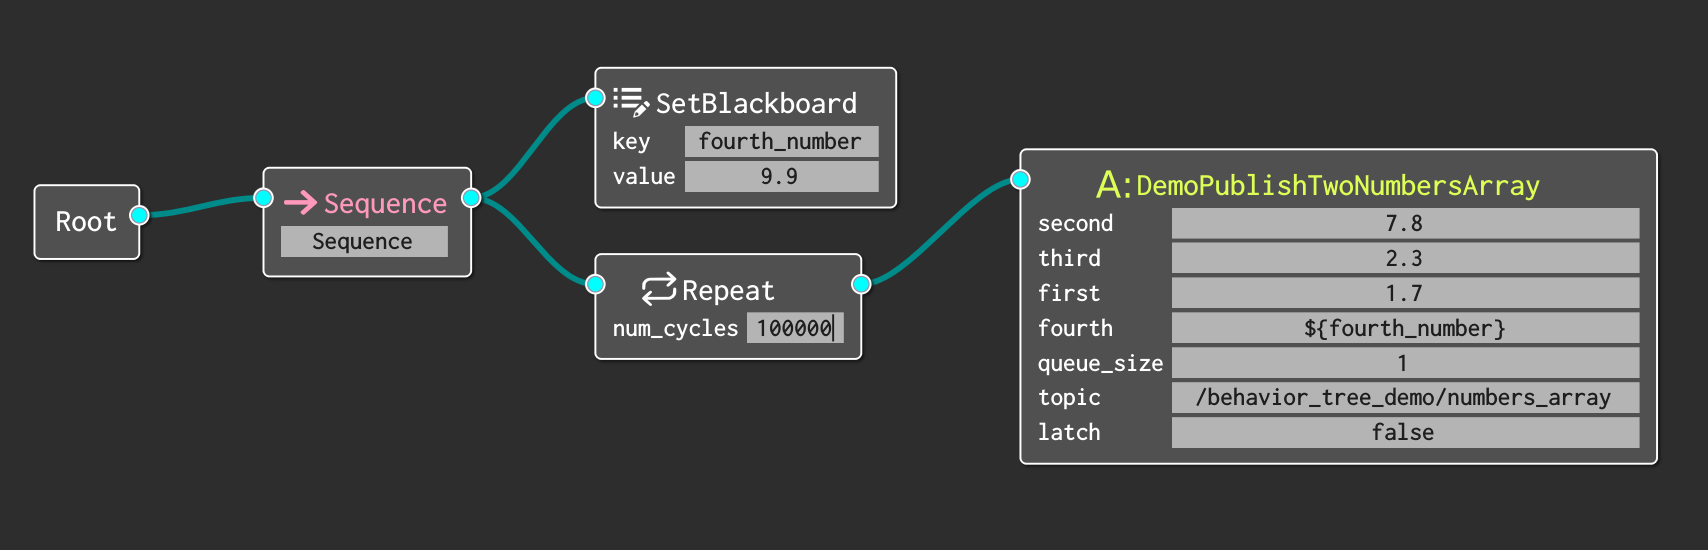
\includegraphics[width=\textwidth]{two_numbers_array_tree.png}
\caption{Tree implementing publisher with user-defined serialization.}
\label{figure:two-numbers-array-tree}
\end{figure}

You are free to build the message in any way you want. You can define as many ports as you need or no ports at all. You can also define just a single port that receives a message of the same type you want to publish. This is an easy way to create a  "normal" publisher.

\end{document}
